 
\documentclass[format=acmsmall]{acmart}

\usepackage{amsmath}
\usepackage{amssymb}
\usepackage{ listings}

\def\F#1#2#3{\mathtt{real\{#1,#2,#3\}}}
\def\eps{\varepsilon}
\def\bbf{\mathbb{F}}
\def\bbr{\mathbb{R}}


\title{Strongly Typed Numerical Computations}


\begin{document}


% \author{Matthieu Martel}
%\affiliation{%
%\institution{Universit\'e de Perpignan Via Domitia}
%\department{Laboratoire de Math\'ematiques et Physique (LAMPS)}
%\streetaddress{52 avenue Paul Alduy}
%\city{Perpignan}
%\postcode{66860}
%\country{France} }
%\email{matthieu.martel@univ-perp.fr}

\begin{abstract}
It is well-known that numerical computations may 
sometimes lead to wrong results because of the accumulation of roundoff errors. In this article,
we propose a ML-like type system (strong, implicit, polymorphic) for numerical computations in
 finite precision, in which the type of an 
arithmetic expression carries information on its accuracy. We  use dependent types 
and a type inference algorithm which, from the user point of view, 
acts like ML  type inference algorithm even if it slightly differs in its implementation. 
While type systems have been widely
used to prevent a large variety of software bugs, to our knowledge, no type system has been targeted 
to address numerical accuracy issues in finite precision computations.
Basically, our type system accepts expressions for which it may ensure a certain accuracy on the result of 
the evaluation and it rejects expressions for which a minimal 
accuracy on the result of the evaluation cannot be inferred. The soundness of the type system is ensured
by a subject reduction theorem and  
we show that our type system does  is able to type usual implementations 
 of usual simple numerical algorithms.
\end{abstract}


%Theory of computation Program analysis
%Theory of computation Type theory
%Mathematics of computing → Arbitrary-precision arithmetic


\begin{CCSXML}
<ccs2012>
<concept>
<concept_id>10002950.10003714.10003715.10003726</concept_id>
<concept_desc>Mathematics of computing~Arbitrary-precision arithmetic</concept_desc>
<concept_significance>500</concept_significance>
</concept>
<concept>
<concept_id>10003752.10003790.10011740</concept_id>
<concept_desc>Theory of computation~Type theory</concept_desc>
<concept_significance>500</concept_significance>
</concept>
<concept>
<concept_id>10003752.10010124.10010138.10010143</concept_id>
<concept_desc>Theory of computation~Program analysis</concept_desc>
<concept_significance>500</concept_significance>
</concept>
</ccs2012>
\end{CCSXML}

\ccsdesc[500]{Theory of computation~Type theory}
\ccsdesc[500]{Mathematics of computing~Arbitrary-precision arithmetic}
\ccsdesc[500]{Theory of computation~Program analysis}

\keywords{numerical accuracy, type inference, dependent types, precision tuning, computer arithmetic}

\maketitle




\section{Introduction}

It is well-known that numerical computations may sometimes lead to wrong results because of the accumulation of 
roundoff errors \cite{Fral17}. 
Recently, much work has been done to detect these accuracy errors in finite precision computations \cite{IEEE754}, by  static \cite{DK14,Gou13,Sal15} or dynamic 
\cite{Dal16} analysis, to find the least
data formats needed to ensure a certain accuracy (precision tuning) \cite{Lal13,Mar17,Ral13} and to optimize the accuracy by program transformation \cite{DMC15,Pal15}.
All these techniques are used late in the software development process, once the programs are entirely written.

In this article, we aim at exploring a different direction. We aim at detecting and correcting numerical accuracy errors at software development time, i.e. during the 
programming phase. From a software engineering point of view, the advantages of our approach are many since it is well-known that late bug detection is time and money 
consuming. We also aim at using intensively used techniques recognized for their ability to discard run-time errors. This choice is motivated by efficiency reasons as well as 
for end-user adopt ability reasons.

We propose a \texttt{ML}-like type system (strong, implicit, polymorphic \cite{Pie02}) for numerical computations in which the type of an 
arithmetic expression carries information on its accuracy. We  use dependent types \cite{Pie04} and a type inference algorithm which, from the user point of view, 
acts like \texttt{ML} \cite{Mal97}  type inference algorithm \cite{Pie02} even if it slightly differs in its implementation. While type systems have been widely
used to prevent a large variety of software bugs, to our knowledge, no type system has been targeted to address numerical accuracy issues in finite precision computations.
Basically, our type system accepts expressions for which it may ensure a certain accuracy on the result of the evaluation and it rejects expressions for which a minimal 
 accuracy on the result of the evaluation cannot be inferred.

In our type system, unification necessitates to solve sets
of constraints made of propositional logic formulas and relations between affine expressions over integers 
(and only integers).
Indeed, these relations remain linear even if the term to be typed contains non-linear computations.
As a consequence, these constraints can be easily checked by a SMT solver 
(we use \texttt{Z3} in practice \cite{Mou08}). 


 Let us insist on the fact that we use a dependent type system. Consequently, the type corresponding to a function of some argument $x$ 
 depends on the type of $x$ itself. 
The soundness of our type system relies on a subject reduction theorem introduced in Section \ref{correct}.
Based on an instrumented operational semantics computing both the finite precision and exact results
of a numerical computation,  this theorem shows that the error on the result of the evaluation of some expression $e$ is less 
than the error predicted by the type of $e$.
Obviously, as any non-trivial type system, our type system is not complete and rejects certain
 programs that would not produce unbounded numerical errors. 
 We show that, in practice,  our type system  is expressive enough  to type implementations 
 of usual simple numerical algorithms \cite{Atk89} such as the trapeze rule, Simpson’s rule, Horner’s scheme, Euler, Runge-Kutta, Newton Raphson algorithms, etc. 
Let us also mention that our type system represents a new application of dependent type theory motivated
by applicative needs. Indeed, dependent types arise naturally in our context since accuracy depends on values.

This article is organized as follows. Section \ref{over} introduces informally our type system and shows how it is used in our implementation of 
a \texttt{ML}-like programming language, \texttt{Numl}.
The formal definition of the types and of the inference rules are given in Section \ref{infe}.
Section \ref{secdeftypes} introduces the type system itself while Section \ref{secdefprim}
introduces the types of the primitives of the language.
A soundness theorem is given in Section \ref{correct}. 
The implementation of the type system is discussed in Section \ref{implem}.
Sections \ref{unif} and \ref{morex} present the unification algorithm and experimental results, respectively.
Section \ref{ieee} discuss the special case of the IEEE754 floating-point arithmetic \cite{IEEE754}.
Section \ref{relate} describes related work 
 and Section \ref{conc} concludes.



\section{Programming with Types for Numerical Accuracy}
\label{over}

In this section, we present informally how our type system works
throughout a programming sequence in our language, \texttt{Numl}.
First of all, we use real 
numbers  $\mathtt{r}\{s,u,p\}$ where $\mathsf{r}$
is the value itself, and $\{s,u,p\}$ the format of $\mathsf{r}$.
The format or a real number is made of a sign $s\in \mathsf{Sign}$ and integers 
$u,p\in \mathsf{Int}$ such that $u$ is the unit in the first place of $\mathsf{r}$,
written $\mathsf{ufp}(\mathsf{r})$ and $p$
the precision.

We have $\mathsf{Sign}=\{0,\oplus,\ominus,\top\}$ and $\mathsf{sign(r)}=0$ if $\mathsf{r}=0$,
$\mathsf{sign(r)}=\oplus$ if $\mathsf{r}>0$ and $\mathsf{sign(r)}=\ominus$ if $\mathsf{r}<0$.
The set $\mathsf{Sign}$ is equipped with the partial order relation $\prec\subseteq \mathsf{Sign}
\times \mathsf{Sign}$ defined by $0\prec \oplus$, $0\prec \ominus$, $\oplus\prec \top$ and 
$\ominus\prec \top$. 

The $\mathsf{ufp}$ of a number $x$ is 
\begin{equation}\label{equfp}
\mathsf{ufp}(x) = \min \big\{ i\in \mathbb{N}\ :\ 2^{i+1} > x\big\} = \lfloor \log_2(x)\rfloor\enspace.
\end{equation}

The term $p$ defines the precision of $\mathsf{r}$. Let $\eps(\mathsf{r})$
be the absolute error on $\mathsf{r}$, we assume that
\begin{equation}
\eps(\mathsf{r})< 2^{u-p+1}\enspace .
\end{equation}
The errors on the numerical constants arising in programs are specified by the user or determined by default by 
the system. The errors on the computed values can be inferred by  propagation of the
initial errors.
Similarly to Equation (\ref{equfp}), we also define the
 \textit{u}nit in the \textit{l}ast \textit{p}lace ($\mathsf{ulp}$) used later in this article.
The $\mathsf{ulp}$ of a number of precision $p$ is defined by
\begin{equation}
 \mathsf{ulp}(x) = \mathsf{ufp}(x) - p+1\enspace .
\end{equation}

\begin{figure}[tb]
\small
\hrule
\vspace{0.2cm}
\centerline{
\begin{tabular}{cccccccccccccccccc}
&Format    &&& Name &&& $p$ &&& $e$ bits  &&& $e_{min}$ &&& $e_{max}$ & \\
\hline
&&&&&&&&&&&&&&&&&\\
&Binary16  &&& Half precision            &&& 11  &&& 5              &&& $-14 $  &&& $+15$ &     \\
&Binary32  &&& Single precision            &&& 24  &&& 8              &&& $-126 $  &&& $+127$ &     \\
&Binary64  &&& Double precision           &&& 53  &&& 11             &&& $-1122 $  &&& $+1223$&     \\
\hspace{0.05cm} & Binary128 &  \hspace{0.05cm}  &  \hspace{0.05cm}  & Quadruple precision            
& \hspace{0.05cm}  &  \hspace{0.05cm}  &113  & \hspace{0.05cm} &  \hspace{0.05cm} & 15             
& \hspace{0.05cm}  & \hspace{0.05cm} & $-16382 $  & \hspace{0.05cm}  & \hspace{0.05cm} & $+16383$ 
&  \hspace{0.05cm}      \\
\end{tabular}}\vspace{0.2cm}
\hrule
\normalsize
\caption{\label{formats}Basic binary IEEE754  formats.}
\end{figure}


For example, the type of $1.234$ is $\F{+}{0}{53}$ since $\mathsf{ufp}(1.234)=0$ and since we assume that, 
by default, the real
numbers have the same precision than in the IEEE754 double precision floating-point format \cite{IEEE754} 
(see Figure \ref{formats}). 
Other formats may be specified by the programmer, as in the example below.
Let us also mention that our type system is independent of a given computer arithmetic. The 
interpreter only needs to implement the formats given by the type system, using floating-point numbers, fixed-point
numbers \cite{MENTOR}, multiple precision numbers\footnote{\tt https://gmplib.org/}, etc
in order to ensure that the finite precision operations are computed exactly.
The special case of the IEEE754 floating-point arithmetic, which introduces additional
errors due to the roundoff of the results of the operations is discussed in Section \ref{ieee}. 
\begin{verbatim}
> 1.234 ;;
- : real{+,0,53} = 1.234000000000000

> 1.234{4};;
- : real{+,0,4} = 1.2
\end{verbatim}
Remark that in our implementation the type information is used by the pretty printer to display 
only the correct digits of a number and a bound on the roundoff error.

Note that
accuracy is not a property of a number but  a number that states how closely a particular floating-point number
matches some ideal true value.
For example, using the basis $\beta=10$ for the sake of simplicity, the floating-point value $3.149$ represents $\pi$ with an accuracy of $3$.
It itself has a precision of $4$. It represents the real number $3.14903$
with an accuracy of $4$. 


As in \texttt{ML}, our type system admits parameterized types \cite{Pie02}. 
\begin{verbatim}
> let f = fun x -> x + 1.0 ;;
val f : real{'a,'b,'c} -> real{<expr>,<expr>,<expr>} = <fun>

> verbose true ;;
- : unit = ()

> f ;;
- : real{'a,'b,'c} -> real{(SignPlus 'a 'b 1 0),
\end{verbatim}
\ \hspace{4.55cm}\texttt{((max 'b 0) +\_ (sigma+ 'a 1)),}

~ \hspace{4.2cm}\texttt{((((max 'b 0) +\_ (sigma+ 'a 1)) }

~ \hspace{4.6cm}\texttt{-\_ (max ('b -\_ 'c) -53))} 

~ \hspace{4.2cm}\texttt{-\_ (iota ('b -\_ 'c) -53))\} = <fun>}

\smallskip

In the example above, the type of \texttt{f} is a function of an argument whose parameterized type is $\F{\texttt{'a}}{\texttt{'b}}{\texttt{'c}}$, where
\texttt{'a}, \texttt{'b} and \texttt{'c} are three type variables. The return type of the function
 \texttt{f} is \texttt{Real\{}$e_0$\texttt{,}$e_1$\texttt{,}$e_2$\texttt{\}} 
where $e_0$, $e_1$ and $e_2$ are arithmetic expressions
containing the variables \texttt{'a}, \texttt{'b} and \texttt{'c}. By default these expressions are not displayed by the system (just like higher order values are not explicitly
displayed in \texttt{ML} implementations) but we may enforce the system to print them. In our implementation we write \texttt{+}, \texttt{-}, \texttt{*} and
\texttt{/} the floating-point operators and \texttt{+\_}, \texttt{-\_}, \texttt{*\_} and
\texttt{/\_} their integer versions. The expressions arising in the type of \texttt{f} are explained in Section \ref{infe}. As shown below, various
applications of \texttt{f} yield results of various types, depending on the type of the argument.
\begin{verbatim}
> f 1.234 ;;
- : real{+,1,53} = 2.234000000000000

> f 1.234{4} ;;
- : real{+,1,5} = 2.2
\end{verbatim}

If the interpreter detects that the result of some computation has no significant digit, then an error is raised. For example, it is well-known that
in IEEE754 double precision $(10^{16} + 1)-10^{16}=0$. Our type system rejects this computation.
\begin{verbatim}
> (1.0e15 + 1.0) - 1.0e15 ;;
- : real{+,50,54} = 1.0 

> (1.0e16 + 1.0) - 1.0e16 ;;
Error: The computed value has no significant digit. Its ufp is 0 but the ulp of the 
certified value is 1 
\end{verbatim}

Last but not least, our type system accepts recursive functions. For example, we have:
\begin{verbatim}
> let rec g x = if x < 1.0 then x else g (x * 0.07) ;;
val g : real{+,0,53} -> real{+,0,53} = <fun>

> g 1.0 ;;
- : real{+,0,53} = 0.07000000000000

> g 2.0 ;;
Error: This expression has type real{+,1,53} but an expression was expected of type
real{+,0,53}
\end{verbatim}

In the above session, the type system unifies the return type of the function with the
type of the conditional. The types of the \texttt{then} and \texttt{else} branches also need to be unified.
Then the return type is \texttt{real\{+,0,53\}} which corresponds to the type of the
value \texttt{1.0} used in the \texttt{then} branch. The type system also unifies the return
type with the type of the argument since the function is recursive. Finally, we obtain that the type
of \texttt{g} is \texttt{real\{+,0,53\} -> real\{+,0,53\}}.
As a consequence, we cannot call \texttt{g}  with an argument whose \textsf{ufp} is greater
than $\mathsf{ufp}(1.0)=0$.
To overcome this limitation, we introduce new comparison operations for real numbers. While
the standard comparison operator \texttt{<} has type \texttt{'a -> 'a -> bool},
the operator \texttt{<\{s,u,p\}} has type \texttt{real\{s,u,p\} -> real\{s,u,p\} -> bool}.
In other words, the compared value are cast in the format $\{s,u,p\}$ before performing the
comparison. Now we can write the code:
\begin{verbatim}
> let rec g x = if x <{*,10,15} 1.0 then x else g (x * 0.07) ;;
val g : real{*,10,15} -> real{*,10,15} = <fun>

> g 2.0 ;;
- : real{*,10,15} = 0.1

> g 456.7 ;;
- : real{*,10,15} = 0.1

> g 4567.8 ;;
Error: This expression has type real{+,12,53} but an expression was expected of 
type real{*,10,15}
\end{verbatim}

Interestingly unstable functions (in the sense that the initial errors grow with 
the number of iterations) are not typable. This is a desirable property of our type system.
\begin{verbatim}
> let rec h n = if (n=0) then 1.0 else 3.33 * (h (n -_ 1)) ;;
Error: This expression has type real{+,-1,-1} but an expression was expected of 
type real{+,-3,-1}
\end{verbatim}

Stable computations should be always accepted by our type system. Obviously,
this is not the case and, as any non-trivial type system, our type system rejects some correct programs.
The challenge is then to accept enough programs to be useful from an end-user point of view.
We end this section by showing a more significant example representative of what our type
system accepts. More examples are given later in this article, in Section \ref{moreex}.

\begin{verbatim}
> let deriv f x h = ((f (x + h)) - (f x)) / h ;;
val deriv : (real{<expr>,<expr>,<expr>} -> real{'a,'b,'c}) 
             -> real{<expr>,<expr>,<expr>} -> real{'d,'e,'f} 
             -> real{<expr>,<expr>,<expr>} = <fun>

> let g x = (x*x) - (5.0*x) + 6.0 ;;
val g : real{'a,'b,'c} -> real{<expr>,<expr>,<expr>} = <fun>

> deriv g 2.0 0.01 ;;
- : real{*,5,51} = -0.9900000000000

> let gprime x = deriv g x 0.01 ;;
val gprime : real{<expr>,<expr>,<expr>} -> real{<expr>,<expr>,<expr>} = <fun>

> let newton x xold f fprime = if ((x-xold)<0.01{*,10,20}) then x 
                               else newton (x-((f x)/(fprime x))) x f fprime ;;
val newton : real{*,10,21} -> real{0,10,20} -> (real{*,10,21} -> real{'a,'b,'c})
             -> (real{*,10,21} -> real{'d,'e,'f}) -> real{*,10,21} = <fun>

> newton 9.0 0.0 g gprime ;;
- : real{*,10,21} = 5.771
\end{verbatim}

%In the programming session above, the function \texttt{rectangle}  implements the rectangle method 
%for numerical integration. It computes the integral $I=\int_a^b f(x)dx$ for a function $f$
%given as parameter (hence \texttt{rectangle} is an higher order function).
In the programming session above, we first define a higher order function \texttt{deriv}
which takes as argument a function and computes its numerical derivative at a given point.
Then we define a function \texttt{g} and compute the value of its derivative at point $2.0$.
Next, by partial application, we build a function computing the derivative of \texttt{g} at any point.
Finally, we define a function \texttt{newton} implementing Newton-Raphson method to find the
zero of a function. The \texttt{newton} function is also an higher order function taking as
argument the function for which a zero has to be found and its derivative. We call the
\texttt{newton} function with our function \texttt{g} and its derivative computed by partial application of the
\texttt{deriv} function. As a result we obtain a root of our polynomial \texttt{g} with a
guaranteed accuracy. Note that while Newton-Raphson method converges quadratically in the exact arithmetic,
numerical errors may perturb the process \cite{DMC15b}.

Obviously, our type system computes the propagation of the errors due to finite precision
but does not take care of the method error intrinsic to the implemented algorithm (Newton-Raphson method
in our case.)
All the programming sessions introduced above are fully interactive in our system, \texttt{Numl},
i.e. the type judgments are obtained instantaneously (about 0.01 second in average following our measurements)
including the most complicated ones of the last session.




\section{The Type System}
\label{infe}

In this section, we introduce the formal definition of our type system for numerical accuracy.
First, in Section \ref{secdeftypes}, we define the syntax of expressions and types and we introduce a set 
of inference rules.
Then we define in Section \ref{secdefprim} the types of the primitives for the operators among real numbers (addition, product, etc.)
These types are crucial in our system since they encode the propagation of the numerical
accuracy information.

\subsection{Expressions, Types and Inference Rules}
\label{secdeftypes}

In this section, we introduce the expressions, types and typing rules for our language.
For the sake of simplicity, the syntax introduced hereafter uses notations \textit{\`a la} lambda calculus
instead of the \texttt{ML}-like syntax employed in Section \ref{over}.
In our system, expressions and types are mutually dependent. They are defined inductively using the grammar of Equation (\ref{eqsyntax}).
\begin{equation}\label{eqsyntax}
\begin{array}{rcl}
\mathsf{Expr}\ni e&::=&\ \mathtt{r}\{s,u,p\}\in \mathsf{Real}_{u,p}\ |\ \mathtt{i}\in \mathsf{Int}
\ |\ \mathtt{b}\in \mathsf{Bool}\ |\ \mathtt{id}\in\mathsf{Id} \\
&&|\  \mathtt{if}\ e_0\ \mathtt{then}\ e_1\ \mathtt{else}\ e_2
\ |\ \lambda x.e
\ |\ e_0\ e_1\ |\ \mathtt{rec}\ f\ x.e\ |\ t\\
&&\\
\mathsf{Typ}\ni t&::=&|\ \mathtt{int}\ |\ \mathtt{bool}\ |\ \mathtt{real\{}i_0,i_1,i_2\mathtt{\}}\ |\ \alpha\ |\ \Pi x:e_0.e_1\\ 
&&\\
\mathsf{IExp}\ni i&::=&|\ \mathtt{int}\ |\ \mathtt{op}\in\mathsf{Id}_\mathsf{I}\ |\ \alpha
\ |\ i_0\ i_1
\end{array}
\end{equation}
In Equation (\ref{eqsyntax}), the $e$ terms correspond to expressions.
Constants are integers $\mathtt{i}\in \mathsf{Int}$, booleans $\mathtt{b}\in \mathsf{Bool}$ and real 
numbers  $\mathtt{r}\{s,u,p\}$ where $\mathsf{r}$
is the value itself, $s\in \mathsf{Sign}$ is the sign and $u,p\in \mathsf{Int}$ the $\mathsf{ufp}$ (see
Equation (\ref{equfp}))
and precision of $\mathtt{r}$. 
We have $\mathsf{Sign}=\{0,\oplus,\ominus,\top\}$ and $\mathsf{sign(r)}=0$ if $\mathsf{r}=0$,
$\mathsf{sign(r)}=\oplus$ if $\mathsf{r}>0$ and $\mathsf{sign(r)}=\ominus$ if $\mathsf{r}<0$.
The set $\mathsf{Sign}$ is equipped with the partial order relation $\prec\subseteq \mathsf{Sign}
\times \mathsf{Sign}$ defined by $0\prec \oplus$, $0\prec \ominus$, $\oplus\prec \top$ and 
$\ominus\prec \top$. The term $p$ defines the precision of $\mathsf{r}$. Let $\eps(\mathsf{r})$
be the absolute error on $\mathsf{r}$, we assume that
\begin{equation}
\eps(\mathsf{r})< 2^{u-p+1}\enspace .
\end{equation}
The errors on the numerical constants arising in programs are specified by the user or determined by default by 
the system. The errors on the computed values can be inferred by  propagation of the
initial errors.


\begin{figure}[tb]
\hrule
\vspace{0.1cm}
$$
\frac{}
     {\Gamma \vdash \texttt{i} :\ \mathtt{int} }\quad\textsc{(Int)}
	 \hspace{2cm}
\frac{}
     {\Gamma \vdash \texttt{b } :\ \mathtt{bool} }\quad\textsc{(Bool)}
$$

$$
\frac{\mathsf{sign}(\texttt{r}) \prec s\quad \mathsf{ufp}(\texttt{r})\le u}
     {\Gamma \vdash \texttt{r\{s,u,p\}}\ :\ \F{s}{u}{p} }\quad\textsc{(Real)}
\hspace{2cm}
\frac{\Gamma(\mathtt{id})=t}
     {\Gamma \vdash \mathtt{id}\ :\ t }\quad\textsc{(Id)}
$$

$$
\frac{
\Gamma \vdash e_0\ :\ \mathtt{bool}\hspace{1cm}\Gamma \vdash e_1\ :\ t_1\hspace{1cm} \Gamma \vdash e_2\ :\ t_2
\hspace{1cm} t=t_1\sqcup t_2}
{\Gamma\vdash \mathtt{if}\ e_0\ \mathtt{then}\ e_1\ \mathtt{else}\ e_2\ :\  t}\quad\textsc{(Cond)}
$$

$$
\frac{\Gamma,x :t_1 \vdash e :  t_2}
     {\Gamma \vdash \lambda x.e : \Pi x:t_1 .  t_2}\quad\textsc{(Abs)}
$$

$$
\frac{\Gamma \vdash e_1 : \Pi x: t_0. t_1\hspace{1cm} \Gamma \vdash e_2 :  t_2
\hspace{1cm} t_2\sqsubseteq t_0
}
     {\Gamma \vdash e_1\ e_2 :  t_2[x\mapsto e_2]}\quad\textsc{(App)}
$$

$$
\frac{\Gamma,x :t_1,f:\Pi.y:t_1.t_2  \vdash e :  t_2}
     {\Gamma \vdash \mathtt{rec}\ f\ x.e : \Pi x:t_1 .  t_2}\quad\textsc{(Rec)}
$$
\vspace{0.1cm}
\hrule
\caption{\label{figtyp}Typing rules for our language.} 
\end{figure}


In Equation (\ref{eqsyntax}), 
identifiers belong to the set $\mathsf{Id}$ and we assume a set of pre-defined identifiers 
$+$, $-$, $\times$, $\le$, $=$, $\ldots$ related to
 primitives for the logical and arithmetic operations.
We write $+$, $-$, $\times$ and $\div$ the operations on real numbers and
  $+\_$, $-\_$, $\times\_$ and $\div\_$ the operations among integers.
The language also admits conditionals, functions $\lambda x.e$, 
applications $e_0\ e_1$ and recursive functions $\texttt{rec}\ f\ x.e$ where
$f$ is the name of the function, $x$ the parameter and $e$ the body.
The language of expressions also includes type expressions $t$ defined by the second production of the grammar 
of Equation (\ref{eqsyntax}).

The definition of expressions and type is mutually recursive.
 Type variables are denoted $\alpha$, $\beta$, $\ldots$
and $\Pi x:e_0.e_1$ is used to introduce dependent types \cite{Pie04}. 
Let us remark that our language does not explicitly contain function types $t_0 \rightarrow t_1$
since they are encoded by means of dependent types. Let $\equiv$ denote the syntactic equivalence, we have
\begin{equation}
t_0\rightarrow t_1  \equiv \Pi x:t_0.t_1\quad\text{with}\ x\ \text{not free in}\ e\enspace .
\end{equation}
For convenience, we also write $\lambda x_0.x_1\ldots x_n.e$ instead of
$\lambda x_0.\lambda x_1\ldots\lambda x_n.e$ and 
$\Pi x_0:t_0.x_1:t_1\ldots x_n:t_n.e$ instead of
$\Pi x_0:t_0.\Pi x_1:t_1\ldots \Pi x_n:t_n.e$.

The types of constants are $\mathtt{int}$, $\mathtt{bool}$ and $\mathtt{real\{}i_0,i_1,i_2\mathtt{\}}$ 
where $i_0$, $i_1$ and $i_2$ 
are integer expressions
denoting the format of the real number. Integer expressions of $\mathsf{IExpr}\subseteq\mathsf{Expr}$ 
are a subset of expressions made of integer numbers, integer primitives of 
$\mathsf{Id}_\mathsf{I}\subseteq \mathsf{Id}$ (such as $+\_$, $\times\_$, etc.), type variables and applications.
Note that this definition restricts significantly the set of expressions which may be written inside
\texttt{real} types.

The typing rules for our system are given in Figure \ref{figtyp}. These rules are mostly classical.
The type judgment $\Gamma\vdash e : t$ means that in the type environment $\Gamma$, the expression
$e$ has type $t$. A type environment $\Gamma : \mathsf{Id}\rightarrow\mathsf{Typ}$ map identifiers to types.
We write $\Gamma\ x:t$ the environment $\Gamma$ in which the variable $x$ has type $t$.
The typing rules \textsc{(Int)} and \textsc{(Bool)} are trivial. Rule \textsc{(Real)} states that
the type of a real number $\texttt{r\{s,u,p\}}$ is  $\F{s}{u}{p}$ assuming that the
actual sign of \texttt{r} is less than $s$ and that the \textsf{ufp} of \texttt{r} is less than $u$.
Following Rule \textsc{(Id)}, an identifier \texttt{id} has type $t$ if $\Gamma(\mathtt{id})=t$.
Rules \textsc{(Cond)}, \textsc{(Abs)} and \textsc{(Rec)} are standard rules for conditionals and abstractions respectively.
The rule for application, \textsc{(App)}, requires that the first expression $e_1$ has type
$\Pi x: t_0. t_1$ (which is equivalent to $t_0\rightarrow t_1$ if $x$ is not free in $t_1$)
and that the argument $e_2$ has some type $t_2\sqsubseteq t_0$. The sub-typing relation $\sqsubset$
is introduced for real numbers. Intuitively, we want to allow the argument of some function
to have a smaller \textsf{ulp} than what we would require if we used $t_0=t_2$ in Rule
\textsc{(App)}, provided that the precision $p$ remains as good with $t_2$ as with $t_0$.
This relaxation allows to type more terms without invalidating the type judgments.
Formally, the relation $\sqsubseteq$ is defined in Equation (\ref{eqlttype}).
\begin{equation}\label{eqlttype}
\F{s_1}{u_1}{p_1} \sqsubseteq \F{s_2}{u_2}{p_2} \iff s_1\sqsubseteq s_2\ \wedge\ u_2 \ge u_1\ \wedge\ p_2 \ge u_1 - u_2 + p_1
\end{equation}
In other words, the sub-typing relation of Equation (\ref{eqlttype}) states that it is
always correct to add zeros before the first significant digit of a number, as illustrated in
Figure \ref{figlt}.
 

\begin{figure}[tb]
  \begin{center}
\hrule
\vspace{0.1cm}
    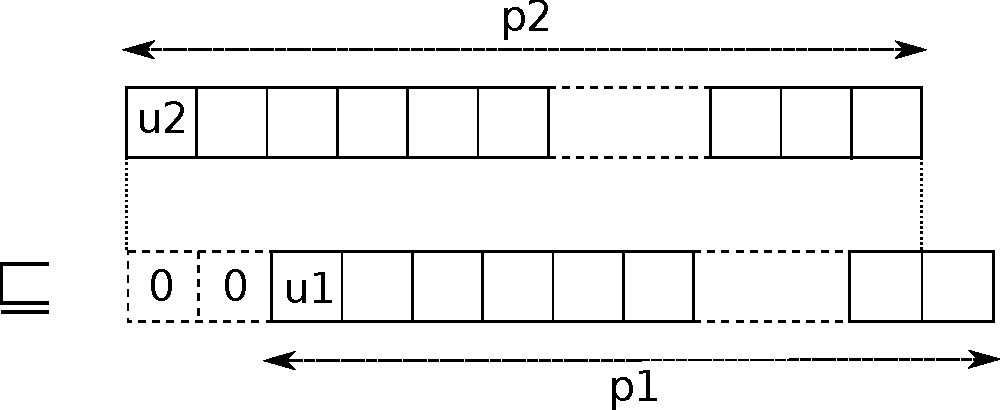
\includegraphics[width=6.5cm]{lttype.pdf}
\vspace{0.1cm}
\hrule
    \caption{    \label{figlt}The sub-typing relation $\sqsubseteq$ of  Equation (\ref{eqlttype}).}
  \end{center}
\end{figure}

\subsection{Types of Primitives}
\label{secdefprim}

In this section, we introduces the types of the primitives of our language.
As mentionned earlier, the arithmetic and logic operators are viewed as functional constants of the language. 
The type of a primitive for an arithmetic operation among integers $\ast\_  \in\{+\_, -\_,\times\_,\div\_\}$ is
\begin{equation}\label{eqtypint}
t_{\ast\_}=\Pi x:\texttt{int}.y:\texttt{int}.\texttt{int}\enspace .
\end{equation}
The type of comparison operators $\Join\in\{=,\not=,<,>,\le,\ge\}$ are polymorphic with the restriction
that they reject the type $\F{s}{u}{p}$ which necessitates special comparison operators:
\begin{equation}\label{eqtyprel}
t_{\Join}=\Pi x:\alpha.y:\alpha.\texttt{bool}\quad \alpha\not=\F{s}{u}{p}\enspace .
\end{equation}
For real numbers, we use comparisons at a given accuracy defined by the operators $\Join_{\{u,p\}}\in
\{<_{\{u,p\}},>_{\{u,p\}}\}$. We have
$$
\begin{array}{c}
t_{\Join_{\{u,p\}}} = \Pi \mathtt{s}:\texttt{int},\mathtt{u}:\texttt{int}, \mathtt{p}:\texttt{int},
\mathtt{s}:\texttt{int}, \mathtt{u}:\texttt{int}, \mathtt{p}:\texttt{int}.\\
\hspace{0.8cm}\F{s}{u}{p+1}\rightarrow\F{s}{u}{p+1}
\rightarrow\mathtt{bool}
\end{array}\enspace .
$$
Remark that the operands of a comparison $\Join_{\{u,p\}}$ must have $p+1$ bits of accuracy.
This is to avoid unstable tests, as detailed in the proof of Lemma \ref{wsubject} in Section \ref{correct}. 
An unstable test is a comparison between two approximate values
such that the result of the comparison is falsened by the approximation error.
For instance, if we reuse an example of Section \ref{over}, in IEEE754 double precision,
the condition $10^{16}+1=10^{16}$ evaluates to \texttt{true}. We need to avoid such situations
in our language in order to preserve our subject reduction theorem (we need the control-flow
be the same in the finite precision and exact semantics).
Let us also note
that our language does not prodive an equality relation $=_{\{u,p\}}$ for \texttt{real} values.
Again this is to avoid unstable tests. Given values $x$ and $y$ of type $\F{s}{u}{p}$,
the programmer is invited to use $|x-y|<2^{u-p+1}$
instead of $x=y$ in order to get rid of the perturbations introduced by the finite precision arithmetic.

%$$
%\begin{array}{c}
%\texttt{+} : \Pi u_1:\texttt{int}. \Pi p_1:\texttt{int}.\Pi u_2:\texttt{int}. \Pi p_2:\texttt{int}.\\
%\quad\F{s_1}{u_1}{p_1}\rightarrow\F{s_2}{u_2}{p_2}\rightarrow\F{??}{u_1+u_2+1}{u_1+u_2+1-\max\big(\mathtt{u_1}-\mathtt{p_1},\mathtt{u_2}-\mathtt{p_2}\big)
%-\iota\big(\mathtt{u_1}-\mathtt{p_1},\mathtt{u_2}-\mathtt{p_2}\big)
%}
%\end{array}
%$$


\begin{figure}[tb]
\hrule			
$$
\begin{array}{c}
\ast\in\{ +,-,\times,\div\}\\
\\
\mathtt{t_\ast} = \Pi \mathtt{s_1}:\texttt{int},\mathtt{u_1}:\texttt{int}, \mathtt{p_1}:\texttt{int},\mathtt{s_2}:\texttt{int}, \mathtt{u_2}:\texttt{int}, \mathtt{p_2}:\texttt{int}.\\
\hspace{0.8cm}\F{s_1}{u_1}{p_1}\rightarrow\F{s_2}{u_2}{p_2}\\
\hspace{3.2cm}
\rightarrow\F{\mathcal{S}_\ast(\mathtt{s_1},\mathtt{u_1},\mathtt{s_2},\mathtt{u_2})}
{\mathcal{U}_\ast(\mathtt{s_1},\mathtt{u_1},\mathtt{s_2},\mathtt{u_2})}
{\mathcal{P}_\ast(\mathtt{s_1},\mathtt{u_1},\mathtt{p_1},\mathtt{s_2},\mathtt{u_2},\mathtt{p_2})}
\end{array}
$$
%\small
$$
\begin{array}{rcl}
\mathcal{U}_+(\mathtt{s_1},\mathtt{u_1},\mathtt{s_2},\mathtt{u_2}))&=&\max(\mathtt{u_1},\mathtt{u_2})
+\sigma_+(\mathtt{s_1},\mathtt{s_2})\\
\mathcal{P}_+(\mathtt{s_1},\mathtt{u_1},\mathtt{p_1},\mathtt{s_2},\mathtt{u_2},\mathtt{p_2}) &=&
\max(\mathtt{u_1},\mathtt{u_2})+\sigma_+(\mathtt{s_1},\mathtt{s_2})-
   \max(\mathtt{u_1}-\mathtt{p_1},\mathtt{u_2}-\mathtt{p_2})-\iota(\mathtt{u_1}-\mathtt{p_1},\mathtt{u_2}-\mathtt{p_2})\\
   \\
\mathcal{U}_-(\mathtt{s_1},\mathtt{u_1},\mathtt{s_2},\mathtt{u_2})) &=&\max(\mathtt{u_1},\mathtt{u_2})
+\sigma_-(\mathtt{s_1},\mathtt{s_2})\\
\mathcal{P}_-(\mathtt{s_1},\mathtt{u_1},\mathtt{p_1},\mathtt{s_2},\mathtt{u_2},\mathtt{p_2}) &=&
\max(\mathtt{u_1},\mathtt{u_2})+\sigma_-(\mathtt{s_1},\mathtt{s_2})-
   \max(\mathtt{u_1}-\mathtt{p_1},\mathtt{u_2}-\mathtt{p_2})-\iota(\mathtt{u_1}-\mathtt{p_1},\mathtt{u_2}-\mathtt{p_2})\\
\\
\\
\mathcal{U}_\times(\mathtt{s_1},\mathtt{u_1},\mathtt{s_2},\mathtt{u_2}))&=&\mathtt{u_1}+\mathtt{u_2}+1\\
\mathcal{P}_\times(\mathtt{s_1},\mathtt{u_1},\mathtt{p_1},\mathtt{s_2},\mathtt{u_2},\mathtt{p_2})&=&
\mathtt{u_1}+\mathtt{u_2}+1-
\max(
\mathtt{u_1}+\mathtt{u_2}+1-\mathtt{p_1},
\mathtt{u_1}+\mathtt{u_2}+1-\mathtt{p_2})-\iota(\mathtt{p_1},\mathtt{p_2})\\
\\
\mathcal{U}_\div(\mathtt{s_1},\mathtt{u_1},\mathtt{s_2},\mathtt{u_2}))&=&\mathtt{u_1}-\mathtt{u_2}+1\\
\mathcal{P}_\div(\mathtt{s_1},\mathtt{u_1},\mathtt{p_1},\mathtt{s_2},\mathtt{u_2},\mathtt{p_2})&=&\mathcal{P}_\times(\mathtt{u_1},\mathtt{p_1},\mathtt{u_2},\mathtt{p_2})-1\\
\\
\iota(x,y)&=&\left\{\begin{array}{l}
1 \ \text{if}\ x=y,\\
0\ \text{otherwise}.
\end{array}\right.
\end{array}
$$
\scriptsize
\vspace{0.2cm}
$$
\begin{array}{ccc}
\mathcal{S}_+&&\mathcal{S}_\times \ \text{and}\ \mathcal{S}_\div
\\
%%%%%%%%%%%%%%%%%%%%%%%%%%%%%%%%%%%%%%%%%%%%%
\begin{array}{c|c|c|c|c}
 \mathtt{s_1} \backslash \mathtt{s_2}
      &\quad 0 \quad& + & - & \quad\top\quad \\
  \hline	  
  \begin{array}{c}
  \\ 0\\ \\
  \end{array}    & 0 & + & - & \top \\
  \hline
  +    & + & + & 
  \begin{array}{c}
  + \ \text{if}\ \mathtt{u_1}<\mathtt{u_2}\\
  - \ \text{if}\ \mathtt{u_2}<\mathtt{u_1}\\
  \top\ \text{otherwise}
  \end{array}&\top\\
  \hline
  -     & - & 
  \begin{array}{c}
  + \ \text{if}\ \mathtt{u_2}<\mathtt{u_1}\\
  - \ \text{if}\ \mathtt{u_1}<\mathtt{u_2}\\
  \top\ \text{otherwise}
  \end{array}
  & - &\top\\
  \hline
  \begin{array}{c}
  \\ \top\\ \\
  \end{array} &\top &\top&\top&\top
\end{array}
&\hspace{1cm}&
\begin{array}{c|c|c|c|c}
   \mathtt{s_1} \backslash \mathtt{s_2}
      &\quad 0 \quad& \quad+\quad & \quad-\quad & \quad\top\quad \\
  \hline	  
  \begin{array}{c}
  \\ 0\\ \\
  \end{array}    & 0 & 0 & 0 & 0 \\
  \hline
  \begin{array}{c}
  \\ +\\ \\
  \end{array}    & 0 &  + & - &\top\\
  \hline
  \begin{array}{c}
  \\ -\\ \\
  \end{array}    & 0 & - & +  &\top\\
  \hline
  \begin{array}{c}
  \\ \top\\ \\
  \end{array} &0 &\top&\top&\top
\end{array}
\end{array}
 $$
\vspace{0.2cm}
 $$
 \begin{array}{ccc}
\mathcal{S}_-&&
\\
\begin{array}{c|c|c|c|c}
 \mathtt{s_1} \backslash \mathtt{s_2}
      &\quad 0 \quad& + & - & \quad\top\quad \\
  \hline	  
  \begin{array}{c}
  \\ 0\\ \\
  \end{array}    & 0 & - & + & \top \\
  \hline
  +    & + &  
  \begin{array}{c}
  - \ \text{if}\ \mathtt{u_1}<\mathtt{u_2}\\
  + \ \text{if}\ \mathtt{u_2}<\mathtt{u_1}\\
  \top\ \text{otherwise}
  \end{array}& +&\top\\
  \hline
  -     & - & - &
  \begin{array}{c}
  - \ \text{if}\ \mathtt{u_2}<\mathtt{u_1}\\
  + \ \text{if}\ \mathtt{u_1}<\mathtt{u_2}\\
  \top\ \text{otherwise}
  \end{array}
  &\top\\
  \hline
  \begin{array}{c}
  \\ \top\\ \\
  \end{array} &\top &\top&\top&\top
\end{array}
&\hspace{2.5cm}&
\begin{array}{cc}
\sigma_+&
\begin{array}{c|cccc}
  & 0 & + & - & \top \\
  \hline
0& 0 & 0  & 0 & 0 \\
+& 0 & 1 & 0 & 1\\
-& 0 & 0 & 1 & 1\\
\top&0&1 & 1 &1 
\end{array}
\\
&\\
\sigma_- &
\begin{array}{c|cccc}
  & 0 & + & - & \top \\
  \hline
0& 0 & 0  & 0 & 0 \\
+& 0 & 0 & 1 & 1\\
-& 0 & 1 & 0 & 1\\
\top&0&1 & 1 &1 
\end{array}
\end{array}
\end{array}
$$
\hrule
\caption{\label{figtypprim}Types of the primitives corresponding to the elementary arithmetic operations.} 
\end{figure}

 
The types of primitives for real arithmetic operators are fundamental in our system since they encode
the propagation of the numerical accuracy information. They are defined in Figure \ref{figtypprim}.
The type $t_\ast$ of some operation $\ast\in\{+,-,\times,\div\}$ is a pi-type with takes
six arguments $\mathsf{s_1,u_1,p_1,s_2,u_2}$ and $\mathsf{p_2}$ of type \texttt{int} corresponding to the sign, \textsf{ufp} and precision of
the two operands of $ast$ and which produces a type
\begin{equation}\label{eqrealtype}
\F{s_1}{u_1}{p_1}\rightarrow\F{s_2}{u_2}{p_2}
\rightarrow\F{\mathcal{S}_\ast(\mathtt{s_1},\mathtt{s_2})}
{\mathcal{U}_\ast(\mathtt{s_1},\mathtt{u_1},\mathtt{s_2},\mathtt{u_2})}
{\mathcal{P}_\ast(\mathtt{u_1},\mathtt{p_1},\mathtt{u_2},\mathtt{p_2})}\enspace .
\end{equation}
In Equation (\ref{eqrealtype}), $\mathcal{S}_\ast$, $\mathcal{U}_\ast$ and $\mathcal{P}_\ast$
are functions which compute the sign, \textsf{ufp} and precision of the result of
the operation $\ast$ in function of  $\mathsf{s_1,u_1,p_1,s_2,u_2}$ and $\mathsf{p_2}$.
These functions are also given in Figure \ref{figtypprim}. They extend the functions
used in \cite{Mar17}.

The functions $\mathcal{S}_\ast$
determine the sign of the result of an operation in function of the signs of the operands and,
for additions and subtractions, in function of the \textsf{ufp}'s of the operands.
The functions $\mathcal{U}_\ast$ compute the \textsf{ufp} of the result.
Remark that $\mathcal{U}_+$ and $\mathcal{U}_-$ use the functions $\sigma_+$ and $\sigma_-$,
respectively. These functions are defined in the bottom right corner of Figure \ref{figtypprim}
to increment the \textsf{ufp} of the result of some addition or subtraction in the relevant cases only.
For example if $a$ and $b$ are two positive real numbers then $\mathsf{ufp}(a+b)$ is possibly 
$\max\big(\mathsf{ufp}(a)+\mathsf{ufp}(b)\big)+1$ but if $a>0$ and $b<0$ then
$\mathsf{ufp}(a+b)$ is not greater than $\max\big(\mathsf{ufp}(a)+\mathsf{ufp}(b)\big)$.
The functions $\mathcal{P}_\ast$ compute the precision of the result. Basically,
they compute the number of bits between the \textsf{ufp} and the \textsf{ulp} 
of the result. 

We end this section by exhibiting some properties of the functions
$\mathcal{P}_\ast$. 
Let
$\eps(x)$ denote the error on $x\in\mathsf{Real}_{u,p}$. We have $\eps(x)< 2^{u-p+1}=\mathsf{ulp}(x)$.
Let us start with the addition. Lemma \ref{lemadd} relates the accuracy of the operands to the accuracy
of the result of an addition between two values $x$ and $y$.

\begin{lemma}\label{lemadd}
Let $x$ and $y$ be two values such that $\eps(x)< 2^{u_1-p_1+1}$ and $\eps(y)< 2^{u_2-p_2+1}$.
Let $z=x+y$ and let
\begin{equation}
\begin{array}{rcl}
u&=&\mathcal{U}_+(s_1,u_1,s_2,u_2)\enspace ,\\
p&=&\mathcal{P}_+(s_1,u_1,p_1,s_2,u_2,p_2)\enspace .
\end{array}
\end{equation}
Then 
\begin{equation}
\eps(z)<2^{u+p-1}\enspace .
\end{equation}
\end{lemma}

\begin{proof}

 The errors on the addition may be bounded
by $e_+=\eps(x)+\eps(y)$. 
Then the most significant bit of the error has weight $\mathsf{ufp}(e_+)$
and the accuracy of the result is $p=\mathsf{ufp}(x + y)-\mathsf{ufp}(e_+)$.
Let 
$$
u=\mathsf{ufp}(x+y)=\max(u_1,u_2)+\sigma_+(s_1,s_2)=\mathcal{U}_+(s_1,u_1,s_2,u_2)
$$
We need to over-approximate $e_+$ in order to ensure $p$. 
We have
$
\eps(x)< 2^{u_1-p_1+1}$ and $\eps(y)< 2^{u_2-p_2+1}
$
and, consequently,
$
e_+ < 2^{u_1-p_1+1}+  2^{u_2-p_2+1}.
$
We introduce the function $\iota(x,y)$ also
defined in Figure \ref{figtypprim} and which is equal to $1$ if $x=y$ and $0$ otherwise.
 We have
$$
\begin{array}{rcl}
\mathsf{ufp}(e_+) &<& \max(u_1-p_1+1,u_2-p_2+1)+\iota(u_1-p_1,u_2-p_2) \\
          &\le& \max(u_1-p_1,u_2-p_2)+\iota(u_1-p_1,u_2-p_2)
\end{array}$$
Let us write
\begin{equation}
p = \max(u_1-p_1,u_2-p_2)-\iota(u_1-p_1,u_2-p_2)=\mathcal{P}_+(s_1,u_1,p_1s_2,u_2,p_2)\enspace .
\end{equation}
We conclude that
$u=\mathcal{U}_+(s_1,u_1,s_2,u_2)$, $p=\mathcal{P}_+(s_1,u_1,p_1s_2,u_2,p_2)$ and
$\eps(z) < 2^{u+p-1}$
\end{proof}

Lemma \ref{lemprod} is similar to Lemma \ref{lemadd}  for the product. 

\begin{lemma}\label{lemprod}
Let $x$ and $y$ be two values such that $\eps(x)< 2^{u_1-p_1+1}$ and $\eps(y)< 2^{u_2-p_2+1}$.
Let $z=x\times y$ and let
\begin{equation}
\begin{array}{rcl}
u&=&\mathcal{U}_\times (s_1,u_1,s_2,u_2)\enspace ,\\
p&=&\mathcal{P}_\times (s_1,u_1,p_1,s_2,u_2,p_2)\enspace .
\end{array}
\end{equation}
Then 
\begin{equation}
\eps(z)<2^{u+p-1}\enspace .
\end{equation}
\end{lemma}


\begin{proof}
For the product, we have
$p	= \mathsf{ufp}(x\times y)-\mathsf{ufp}(e_\times)$ with $e_\times=x\cdot \eps(y)+y\cdot \eps(x)+\eps(x)\cdot\eps(y)$. 
Let
$$
u=u_1+u_2+1=\mathcal{U}_\times (s_1,u_1,s_2,u_2)\enspace .
$$

We have, by definition of $\mathsf{ufp}$,
$
2^{u_1} \le x < 2^{u_1+1}\quad\text{and}\quad 2^{u_2} \le y< 2^{u_2+1}\enspace.
$
Then $e_\times$ may be bound by
\begin{equation}\label{eqproof1}
\begin{array}{rcl}
e_\times &<& 2^{u_1+1}\cdot 2^{u_2-p_2+1} + 2^{p_2+1}\cdot 2^{u_1-p_1+1}+ 2^{u_1-p_1+1}\cdot 2^{u_2-p_2+1}\\
            &=& 2^{u_1+u_2-p_2+2}+ 2^{u_1+u_2-p_1+2}+ 2^{u_1+u_2-p_1-p_2+2} \enspace.
\end{array}
\end{equation}
Since $u_1+u_2-p_1-p_2+2< u_1+u_2-p_1+2$ and $u_1+u_2-p_1-p_2+2< u_1+u_2-p_2+2$, 
we may get rid of the last term of Equation (\ref{eqproof1}) and we
obtain that
$$
\begin{array}{rcl}
\mathsf{ufp}(e_\times) &<& \max(u_1+u_2-p_1+2,u_1+u_2-p_2+2)+\iota(p_1,p_2)\\
&\le & \max(u_1+u_2-p_1+1,u_1+u_2-p_2+1)+\iota(p_1,p_2)\enspace.
\end{array}
$$
Let us write
\begin{equation}
p = \max(u_1+u_2-p_1+1,u_1+u_2-p_2+1)-\iota(p_1,p_2)=\mathcal{P}_\times(s_1,u_1,p_1s_2,u_2,p_2)\enspace .
\end{equation}
We conclude that
$u=\mathcal{U}_\times(s_1,u_1,s_2,u_2)$, $p=\mathcal{P}_\times(s_1,u_1,p_1s_2,u_2,p_2)$ and
$\eps(z) < 2^{u+p-1}$
\end{proof}

Note that, by reasoning on the exponents of the values, the constraints resulting from a product become linear.
The equations for the subtraction and division are almost identical to the equations for the addition and product, 
respectively. Note that the result of a division has one less bit than the result of a product.
This is due to the fact that, even in the operands are finite numbers, the result of the
division may be irrational and possibly needs to be truncated.
We conclude this section with the following theorem which summarize the properties of the types
of the result of the four elementary operations.

\begin{theorem}\label{thop}
Let $x$ and $y$ be two values such that $\eps(x)< 2^{u_1-p_1+1}$ and $\eps(y)< 2^{u_2-p_2+1}$ and
let $\ast\in\{ +,-,\times,\div\}$ be an elementary operation.
Let $z=x\ast y$ and let
\begin{equation}
\begin{array}{rcl}
u&=&\mathcal{U}_\ast (s_1,u_1,s_2,u_2)\enspace ,\\
p&=&\mathcal{P}_\ast (s_1,u_1,p_1,s_2,u_2,p_2)\enspace .
\end{array}
\end{equation}
Then 
\begin{equation}
\eps(z)<2^{u+p-1}\enspace .
\end{equation}
\end{theorem}

\begin{proof}
The cases of the addition and product correspond to Lemma \ref{lemadd} and Lemma \ref{lemprod}, respectively.
The cases of the subtraction and  division are similar to the former ones.
\end{proof}






\begin{figure}[tb]
\hrule
\vspace{0.1cm}
$$
\frac{|\mathtt{r}-v_\bbf|< 2^{u-p+1} \quad \mathsf{ufp}(\mathtt{r})\le u\quad \mathsf{sign}(v_\bbf)\prec s}
     {\mathtt{r\{s,u,p\} } \rightarrow_\bbf v_\bbf}\quad\textsf{(FVal)}
\hspace{1cm}
\frac{v_\bbr=\mathtt{r}}
     {\mathtt{r\{s,u,p\} } \rightarrow_\bbr v_\bbr}\quad\textsf{(RVal)}
$$

$$
\frac{e_0 \rightarrow e_0'}
     {e_0\ast e_1 \rightarrow e_0'\ast e_1}\quad\textsf{(Op1)}
\hspace{1cm}
\frac{e_1 \rightarrow e_1'}
     {v\ast e_1 \rightarrow v\ast  e_1'}\quad\textsf{(Op2)}\hspace{1cm}\ast\in\{+,-,\times,\div,+\_,-\_,\times\_,\div_\_\}
$$


$$
\frac{v=v_0\ast v_1}
     {v_0\ast v_1 \rightarrow v}\quad\textsf{(Op)}\hspace{1cm}\ast\in\{+,-,\times,\div,+\_,-\_,\times\_,\div_\_\}
$$



$$
\frac{e_0 \rightarrow e_0'}
     {e_0\Join e_1 \rightarrow e_0'\Join e_1}\quad\textsf{(Cmp1)}
\hspace{1cm}
\frac{e_1 \rightarrow e_1'}
     {v\Join e_1 \rightarrow v\Join e_1'}\quad\textsf{(Cmp2)}
\hspace{1cm}\Join\in\{<_{\{u,p\}},>_{\{u,p\}},<,>\}
$$

$$
\frac{ b=(v_0^\bbf- v_1^\bbf\Join 2^{u-p+1})
}
     {v_0\Join_{\{u,p\}} v_1 \rightarrow_\bbf b}\quad\textsf{(FCmp)}
\hspace{1cm}%\Join\in\{<_{\{u,p\}},>_{\{u,p\}}\}
%$$
%$$
\frac{b=(v_0\Join v_1)
}
     {v_0\Join_{\{u,p\}} v_1 \rightarrow_\bbr b}\quad\textsf{(RCmp)}
\hspace{1cm}\Join\in\{<_{\{u,p\}},>_{\{u,p\}}\}
$$

$$
\frac{b=v_0\Join v_1}
     {v_0\Join v_1 \rightarrow b}\quad\textsf{(ACmp)}
\hspace{1cm}\Join\in\{=,\not=,<,>,\le,\ge\}
$$


$$
\frac{e_1 \rightarrow e_1'}
     {e_0\ e_1 \rightarrow e_0\ e_1'}\quad\textsf{(App1)}
\hspace{1cm}
\frac{e_0 \rightarrow e_0'}
     {e_0\ v \rightarrow e_0'\ v}\quad\textsf{(App2)}
\hspace{1cm}
%\frac{}
     {(\lambda x.e)\ v\rightarrow e\langle v/x\rangle}\quad\textsf{(Red)}
$$
$$
\frac{e_0 \rightarrow e_0'}
     {\mathtt{if}\ e_0\ \mathtt{then}\ e_1\ \mathtt{else}\ e_2
      \rightarrow \mathtt{if}\ e_0'\ \mathtt{then}\ e_1\ \mathtt{else}\ e_2
     }\quad\textsf{(Cond)}
$$

$$
\frac{v=\mathtt{true}}
     {\mathtt{if}\ v\ \mathtt{then}\ e_1\ \mathtt{else}\ e_2
      \rightarrow  e_1
     }\quad\textsf{(CondTrue)}
\hspace{1cm}
\frac{v=\mathtt{false}}
     {\mathtt{if}\ v\ \mathtt{then}\ e_1\ \mathtt{else}\ e_2
      \rightarrow  e_2
     }\quad\textsf{(CondFalse)}
$$

$$
     {\mathtt{rec}\ f\ x.e} \rightarrow \lambda x.e\langle \mathtt{rec}\ f\ x.e/f\rangle \quad\textsc{(Rec)}
$$

\vspace{0.1cm}
\hrule
\caption{\label{figsem}Operational semantics for our language.} 
\end{figure}


\section{Soundness of the Type System}
\label{correct}

In this section, we introduce a subject reduction theorem proving the consistency of our type system.
We use two operational semantics $\rightarrow_\bbf$ and $\rightarrow_\bbr$ for the finite precision
and exact arithmetics, respectively. 
The exact semantics is used for proofs. Obviously, in practice, only
the finite precision semantics is implemented.
We write $\rightarrow$ whenever a reduction rule holds for either
$\rightarrow_\bbf$ or $\rightarrow_\bbr$ (in this case, we assume that the same semantics $\rightarrow_\bbf$
or $\rightarrow_\bbr$ is used in the lower and upper parts of the same sequent).
The finite precision and exact semantics are  
displayed in Figure \ref{figsem}.
They concern the subset of the language of Equation (\ref{eqsyntax}) which do not deal with types
and defined by
 
\begin{equation}
\label{eqsyntax2}
\begin{array}{rcl}
\mathsf{EvalExpr}\ni e&::=&\ \mathtt{r}\{s,u,p\}\in \mathsf{Real}_{u,p}\ |\ \mathtt{i}\in \mathsf{Int}
\ |\ \mathtt{b}\in \mathsf{Bool}\ |\ \mathtt{id}\in\mathsf{Id} \\
&&|\  \mathtt{if}\ e_0\ \mathtt{then}\ e_1\ \mathtt{else}\ e_2
\ |\ \lambda x.e
\ |\ e_0\ e_1\ |\ \mathtt{rec}\ f\ x.e
|\ e_0\ \ast\ e_1
\end{array}\enspace .
\end{equation}

In Equation (\ref{eqsyntax2}), $\ast$ denotes an arithmetic operator
$\ast\in\{+,-,\times,\div,+\_,-\_,\times\_,\div\_\}$.
In Figure \ref{figsem}, Rule \textsc{(FVal)} of $\rightarrow_\bbf$ transforms a syntactic element 
describing a real number
$\mathtt{r\{s,u,p\} }$ in a certain format into a value $v_\bbf$.
The finite precision value $v_\bbf$ is an approximation of $\mathtt{r}$ with
an error less than the \textsf{ulp} of $\mathtt{r\{s,u,p\} }$.
In the semantics $\rightarrow_\bbr$, the real number $\mathtt{r\{s,u,p\} }$ simply
produces the value \texttt{r} without any approximation by Rule \textsf{(RVal)}.
Rules \textsf{(Op1)} and  \textsf{(Op2)} evaluate the expressions corresponding to the operands
of some binary operation and Rule  \textsf{(Op)} performs an operation $\ast\in\{+,-,\times,\div,+\_,-\_,\times\_,\div_\_\}$
between two values $v_0$ and $v_1$. 

Rules \textsf{(Cmp1)}, \textsf{(Cmp2)} and \textsf{(ACmp)} deal with comparisons.
They are similar to Rules \textsf{(Op1)}, \textsf{(Op2)} and \textsf{(Op)} described earlier.
Note that the operators $<,\ >,\ =,\ \not=$ concerned by Rule \textsf{(ACmp)} are polymorphic
excepted that they do not accept arguments of type \texttt{real}.
Rules \textsf{(FCmp)} and \textsf{(RCmp)} are for the comparison of \texttt{real} values. Rule 
\textsf{(FCmp)} is designed 
to avoid unstable tests by requiring that the distance between the 
two compared values is greater than the \textsf{ulp} of the format in which the comparison is
done. With this requirement, a condition cannot be invalidated by the roundoff errors.
Let us also note  that, with this definition, $x<_{u,p} y \not\Rightarrow y>_{u,p} x$
or $x>_{u,p} y \not\Rightarrow y<_{u,p} x$. For the semantics $\rightarrow_\bbr$, Rule \textsf{(RCmp)}
simply compares the exact values.

The other rules are standard and are identical in $\rightarrow_\bbf$
and $\rightarrow_\bbr$. Rules \textsf{(App1)}, \textsf{(App2) and \textsf{(Red)}}
are for applications and Rule \textsf{(Rec)} is for recursive functions. 
 We write $e\langle v/x\rangle$ the term $e$ in which $v$ has been substituted
to the free occurrences of $x$. Finally, Rules \textsf{(Cond)}, \textsf{(CondTrue)} and \textsf{(CondFalse)} 
are for conditionals.


\begin{figure}[tb]
\hrule
\vspace{0.1cm}
$$
\frac{}
     {\Gamma \models (\texttt{i},\texttt{i}) :\ \mathtt{int} }\quad\textsc{(Int)}
	 \hspace{1cm}
\frac{}
     {\Gamma \models (\texttt{b},\texttt{b}) :\ \mathtt{bool} }\quad\textsc{(Bool)}
\hspace{1cm}
\frac{\Gamma(\mathtt{id})=t}
     {\Gamma \models (\mathtt{id},\mathtt{id})\ :\ t }\quad\textsc{(Id)}
$$

$$
\frac{\mathsf{sign}(\texttt{r}) \prec s\quad \mathsf{ufp}(\texttt{r})\le u}
     {\Gamma \models (\texttt{r\{s,u,p\}},\texttt{r\{s,u,p\}})\ :\ \F{s}{u}{p} }\quad\textsc{(SReal)}
\hspace{0.5cm}
\frac{|v_\bbr-v_\bbf|<2^{u-p+1}}
     {\Gamma \models (v_\bbf,v_\bbr)\ :\ \F{s}{u}{p} }\quad\textsc{(VReal)}
$$

$$
\frac{\Gamma \models (e_{1\bbf},e_{1\bbr}) : \F{s_1}{u_1}{p_1}\hspace{0.5cm} 
      \Gamma \models (e_{2\bbf},e_{2\bbr}) : \F{s_1}{u_1}{p_1}
\hspace{0.5cm}\ast\in\{+,-,\times,\div\}
}
     {\Gamma \models (e_{1\bbf}\ast e_{2\bbf},e_{1\bbr}\ast e_{2\bbr}) :  
\F{\mathcal{S}_\ast(s_1,u_1,s_2,u_2)}{\mathcal{U}_\ast(s_1,u_1,s_2,u_2)}{\mathcal{P}_\ast(s_1,u_1,p_1,s_2,u_2,p_2)}
}\quad\textsc{(ROp)}
$$

$$
\frac{\Gamma \models (e_{1\bbf},e_{1\bbr}) : \F{s_1}{u}{p+1}\hspace{0.5cm} 
      \Gamma \models (e_{2\bbf},e_{2\bbr}) : \F{s_1}{u}{p+1}
\hspace{0.5cm}\ast\in\{<,>\}
}
     {\Gamma \models (e_{1\bbf}\Join_{u,p} e_{2\bbf},e_{1\bbr}\Join_{u,p} e_{2\bbr}) :  
\mathtt{bool}
}\quad\textsc{(RCmp)}
$$

$$
\frac{\Gamma \models (e_{1\bbf},e_{1\bbr}) : \mathtt{int}\hspace{0.5cm} 
      \Gamma \models (e_{2\bbf},e_{2\bbr}) : \mathtt{int}
\hspace{0.5cm}{\ast\_}\in\{+\_,-\_,\times\_,\div\_\}
}
     {\Gamma \models (e_{1\bbf}\ {\ast\_}\ e_{2\bbf},e_{1\bbr}\ {\ast\_}\ e_{2\bbr}) :  
\mathtt{int}
}\quad\textsc{(IntOp)}
$$

$$
\frac{\Gamma \models (e_{1\bbf},e_{1\bbr}) : t\hspace{0.5cm} 
      \Gamma \models (e_{2\bbf},e_{2\bbr}) : t\hspace{0.5cm}t\not=\F{s}{u}{p}
\hspace{1cm}\Join\in\{=,\not=,<,>,\le,\ge\}
}
     {\Gamma \models (e_{1\bbf}\Join e_{2\bbf},e_{1\bbr}\Join e_{2\bbr}) :  
\mathtt{bool}
}\quad\textsc{(ACmp)}
$$


$$
\frac{
\Gamma \models (e_{0\bbf},e_{0\bbr})\ :\ \mathtt{bool}\hspace{0.5cm}\Gamma \models (e_{1\bbf},e_{1\bbr})\ :\ t_1
\hspace{0.5cm} \Gamma \models (e_{2\bbf},e_{2\bbr})\ :\ t_2
\hspace{0.5cm} t=t_1\sqcup t_2}
{\Gamma\models (\mathtt{if}\ e_{0\bbf}\ \mathtt{then}\ e_{\bbf}1\ \mathtt{else}\ e_{2\bbf},
                \mathtt{if}\ e_{0\bbr}\ \mathtt{then}\ e_{1\bbr}\ \mathtt{else}\ e_{2\bbr})\ :\  t}\quad\textsc{(Cond)}
$$

$$
\frac{\Gamma,x :t_1 \models (e_\bbf,e_\bbr) :  t_2}
     {\Gamma \models (\lambda x.e_\bbf,\lambda x.e_\bbr) : \Pi x:t_1 .  t_2}\quad\textsc{(Abs)}
$$

$$
\frac{\Gamma \models (e_{1\bbf},e_{1\bbr}) : \Pi x: t_0. t_1\hspace{1cm} \Gamma \models (e_{2\bbf},e_{2\bbr}) :  t_2
\hspace{1cm} t_2\sqsubseteq t_0
}
     {\Gamma \models (e_{1\bbf}\ e_{2\bbf},e_{1\bbr}\ e_{2\bbr}) :  t_2[x\mapsto e_2]}\quad\textsc{(App)}
$$

$$
\frac{\Gamma,x :t_1,f:\Pi.y:t_1.t_2  \models (e_\bbf,e_\bbr) :  t_2}
     {\Gamma \models (\mathtt{rec}\ f\ x.e_\bbf,\mathtt{rec}\ f\ x.e_\bbr) : \Pi x:t_1 .  t_2}\quad\textsc{(Rec)}
$$
\vspace{0.1cm}
\hrule
\caption{\label{figmod}Inference rules for the simulation relation $\models$ used in our subject reduction theorem.} 
\end{figure}


The rest of this section is dedicated to our subject reduction theorem.
First of all, we need to relate the traces of $\rightarrow_\bbf$ and $\rightarrow_\bbr$.
We introduce new judgments 
\begin{equation}\label{eqmod}
\Gamma \models (e_\bbf,e_\bbr)\ :\ t\enspace . 
\end{equation}
Intuitively, Equation (\ref{eqmod}) means that  expression $e_\bbf$ simulates 
$e_\bbr$ up to accuracy $t$. In this case, $e_\bbf$
is syntactically equivalent to $e_\bbr$ up to the values which, in $e_\bbf$,
are approximations of the values of $e_\bbr$. The quantification of the approximation
is given by type $t$. 

Formally, $\models$ is defined in Figure \ref{figmod}. These rules are similar to the typing rules
rules of Figure \ref{figtyp} excepted that they operate on pairs $(e_\bbf,e_\bbr)$.
They are also designed for the language of Equation (\ref{eqsyntax2}) and, consequently,
deal with the elementary arithmetic operations $+,\ -,\ \times$ and $\div$ as well
as the comparison operators. 
The difference between the rules of Figure \ref{figtyp} and Figure \ref{figmod} is
in Rule \textsf{(VReal)} which states that a  \texttt{real} value $v_\bbr$
is correctly simulated by a value $v_\bbf$ up to accuracy $\F{s}{u}{p}$ if
$|v_\bbr-v_\bbf|<2^{u-p+1}$. 
It is easy to show, by examination of the rules of figures \ref{figtyp} and \ref{figmod}
that
\begin{equation}
\Gamma \models (e_\bbf,e_\bbr)\ :\ t\ \Longrightarrow\Gamma \vdash e_\bbf\ :\ t\enspace .
\end{equation}

We introduce now Lemma \ref{wsubject} which states the soundness of the type system for one
reduction step. 
Basically, this lemma states that types are preserved by reduction and that 
concerning the values of type \texttt{real}, the distance between the finite precision value
and the exact value is less than the \textsf{ulp} given by the format of the type.


\begin{lemma}[Weak subject reduction]
\label{wsubject}
If\ $\Gamma \models (e_\bbf,e_\bbr)\ : t$ and if  $e_\bbf\rightarrow_\bbf e_\bbf'$ and
$e_\bbr\rightarrow_\bbr e_\bbr'$ then $\Gamma \models (e_\bbf',e_\bbr')\ : t$. 
%In addition,
%if $e\equiv v$ and $t=\mathtt{real\{s,u,p\}}$ then $|\mathbb{R}(v)-\mathbb{F}(v)|< 2^{u-p+1}$.
\end{lemma} 

\begin{proof}
By induction on the structure of expressions
and case examination on the possible transition rules of Figure \ref{figsem}.
\begin{itemize}
%%%%%%%%%%%%
\item If $e_\bbf\equiv e_\bbr\equiv\mathtt{r\{s,u,p\}}$ then %, from  Rule \textsf{(SReal)} 
%of Figure \ref{figmod}, 
$\Gamma \models (\texttt{r\{s,u,p\}},\texttt{r\{s,u,p\}})\ :\ \F{s}{u}{p} $ and,
from the reduction rules \textsf{(FVal)} and \textsf{(RVal)} of Figure \ref{figsem},
$\mathtt{r\{s,u,p\}} \rightarrow_\bbf v_\bbf$ and
$\mathtt{r\{s,u,p\}} \rightarrow_\bbr v_\bbr$
with $|v_\bbf-v_\bbf|< 2^{u-p+1}$.
So $\Gamma\models (v_\bbf,v_\bbr)\ :\ \F{s}{u}{p} $.
%%%%%%%%%%%
\item If $e_\bbf\equiv e_{0\bbf}\ast e_{1\bbf}$ and $e_\bbr\equiv e_{0\bbr}\ast e_{1\bbr}$
 then several cases must be distinguished. 
\begin{itemize}
\item If $e_\bbf\equiv v_{0\bbf}\ \ast\ v_{1\bbf}$ and $e_\bbr\equiv v_{0\bbr}\ \ast\ v_{1\bbr}$ then, by induction hypothesis,
$\Gamma\models (v_{0\bbf},v_{0\bbr})\ :\mathtt{real\{s_0,u_0,p_0\}}$, 
$\Gamma\models (v_{1\bbf},v_{1\bbr})\ :\mathtt{real\{s_1,u_1,p_1\}}$ and, consequently, from
Rule \textsc{(VReal)},
\begin{equation}\label{eqproof2}
|v_{0\bbr}-v_{0\bbf}|<2^{u_0-p_0+1}\quad \text{and}\quad|v_{1\bbr}-v_{1\bbf}|<2^{u_1-p_1+1}\enspace. 
\end{equation}
Following Figure \ref{figtypprim}, the type $t$ of $e$ is
$$
\begin{array}{rcl}
t&=& \big(\Pi \mathtt{s_1}:\texttt{int},\mathtt{u_1}:\texttt{int}, \mathtt{p_1}:\texttt{int},
       \mathtt{s_2}:\texttt{int},\mathtt{u_2}:\texttt{int}, \mathtt{p_2}:\texttt{int}.\\
%\hspace{0.8cm}
&&\quad \F{s_1}{u_1}{p_1}\rightarrow\F{s_2}{u_2}{p_2}\rightarrow \\
&&\quad \rightarrow\F{\mathcal{S}_\ast(\mathtt{s_1},\mathtt{u_1},\mathtt{s_2},\mathtt{u_2})}
{\mathcal{U}_\ast(\mathtt{s_1},\mathtt{u_1},\mathtt{s_2},\mathtt{u_2})}
{\mathcal{P}_\ast(\mathtt{s_1},\mathtt{u_1},\mathtt{p_1},\mathtt{s_2},\mathtt{u_2},\mathtt{p_2})}\\
&&\big)\ \mathtt{s_1\ u_1\ p_1\ s_2\ u_2\ p_2}\enspace ,\\
&=&\F{\mathcal{S}_\ast(\mathtt{s_1},\mathtt{u_1},\mathtt{s_2},\mathtt{u_2})}
{\mathcal{U}_\ast(\mathtt{s_1},\mathtt{u_1},\mathtt{s_2},\mathtt{u_2})}
{\mathcal{P}_\ast(\mathtt{s_1},\mathtt{u_1},\mathtt{p_1},\mathtt{s_2},\mathtt{u_2},\mathtt{p_2})}\\
&=&\mathtt{real\{s,u,p\}}
\end{array}
$$
By Rule \textsc{(Op)}, $e\rightarrow_\bbf v_\bbf$ and $e\rightarrow_\bbr v_\bbr$ and, 
by Theorem \ref{thop}, with  the assumptions of Equation (\ref{eqproof2}), we know that $|v_\bbr-v_\bbf|<2^{u-p+1}$.
Consequently, $\Gamma\models (v_\bbf,v_\bbr)\ :\ \F{s}{u}{p}$.
\item If $e_\bbf\equiv v_{0\bbf}\ \ast\ v_{1\bbf}$ and $e_\bbr\equiv v_{0\bbr}\ \ast\ v_{1\bbr}$
 with $\Gamma\models( v_0, v_1)\ :\ \mathtt{int}$ then,
by Rule \textsf{(Op)}, $e\rightarrow (v,v)$ and,
by Equation (\ref{eqtypint}), $\Gamma\vdash v\ :\ \mathtt{int}$.
If $e\equiv e_0\ast e_1$ then, by Rule $\textsf{(Op1)}, e\rightarrow e_0\ast e_1'$ and we conclude by
induction hypothesis. The case $e\equiv e_0\ast\ v_1$ is similar to the former one.
\end{itemize}
%%%%%%%%%%%%%%%%%%%%%%%%%%%%%%%%%%%%%%%%%
\item If $e_\bbf\equiv e_{0\bbf}\Join_{u,p} e_{1\bbf}$ and $e_\bbr\equiv e_{0\bbr}\Join_{u,p} e_{1\bbr}$
then several cases have to be examined.
\begin{itemize}
\item If $e_\bbf\equiv v_{0\bbf}\Join_{u,p} v_{1\bbf}$ and
$e_\bbr\equiv v_{0\bbr}\Join_{u,p} v_{1\bbr}$
 then by rules \textsf{(FCmp)} and \textsf{(RCmp)}
$e_\bbf\rightarrow_\bbf b_\bbf$, $e_\bbr\rightarrow_\bbr b_\bbr$ with
\begin{equation}\label{eqproofjoin}
b_\bbf=     v_{0\bbf}- v_{1\bbf} \Join_{\{u,p\}} 2^{u-p+1}
\quad\text{and}\quad
b_\bbf=     v_{0\bbr} -v_{1\bbr} \Join_{\{u,p\}} 0 \enspace .
\end{equation}
By rule \textsf{(RCmp)} of Figure \ref{figmod}, $\Gamma\models (v_{0\bbf},v_{1\bbf})\ :\ \F{s}{u}{p}$
and $\Gamma\models (v_{0\bbr},v_{1\bbr})\ :\ \F{s}{u}{p}$.
Consequently,
\begin{equation}
|v_{0\bbr}-v_{0\bbf}| < 2^{u-p+1}\quad\text{and}\quad |v_{1\bbr}-v_{1\bbf}| < 2^{u-p+1}
\end{equation}
By combining equations (\ref{eqproofjoin}) and (\ref{eqproofjoin}), we obtain that
\begin{equation}
|(v_{0\bbr}-v_{1\bbr})-(v_{0\bbf}-v_{1\bbf})| < 2^{u-p}\enspace .
\end{equation}
Consequently, $b_\bbf=b_\bbr$ and we conclude that $\Gamma\models (b_\bbf,b_\bbr)\ : \mathtt{bool}$.
\item The other cases for $e_\bbf\equiv e_{0\bbf}\Join_{u,p} e_{1\bbf}$
are similar to the cases $e_\bbf\equiv v_{0\bbf}\ast v_{1\bbf}$ examined previously.
\end{itemize}
\item The other cases simply follow the structure of the terms, by application of the induction hypothesis.
\end{itemize}
\end{proof}



Let $\rightarrow^*$ denote the reflexive transitive closure of $\rightarrow$.
Theorem \ref{subject} expresses the soundness of our type system for sequences of reduction
of arbitrary length.

\begin{theorem}[Subject reduction]
\label{subject}
If\ $\Gamma \vdash e\ : t$ and $e\rightarrow^* e'$ then $\Gamma \vdash e'\ : t$. In addition,
if $e\equiv v$ and $t=\mathtt{real\{s,u,p\}}$ then $|\mathbb{R}(v)-\mathbb{F}(v)|< 2^{u-p+1}$.
\end{theorem} 

\begin{proof}
By induction on the length of the reduction sequence, using Lemma \ref{wsubject}.
\end{proof}

Theorem \ref{subject} assert the soundness of our type system. It states that the evaluation of an expression of type $\F{s}{u}{p}$ yields
a result of accuracy $2^{u-p+1}$.





\begin{figure}[tb]
{\tt \small
\hrule
\vspace{0.2cm}
\begin{lstlisting}[mathescape]
$\mathbf{let}$ $\mathbf{rec}$ unifyReal $\mathtt{s_1}$ $\mathtt{u_1}$ $\mathtt{p_1}$ $\mathtt{s_2}$ $\mathtt{u_2}$ $\mathtt{p_2}$ = $\mathbf{match}$ (!$\mathtt{s_1}$,!$\mathtt{u_1}$,!$\mathtt{p_1}$) $\mathbf{with}$
  ($\mathbf{in}$t($\mathtt{s_1}'$),$\mathbf{in}$t($\mathtt{u_1}'$),$\mathbf{in}$t($\mathtt{p_1}'$)) $\rightarrow$  
    ($\mathbf{match}$ (!$\mathtt{s_2}$,!$\mathtt{u_2}$,!$\mathtt{p_2}$) $\mathbf{with}$
       ($\mathbf{in}$t($\mathtt{s_2}'$),$\mathbf{in}$t($\mathtt{u_2}'$),$\mathbf{in}$t($\mathtt{p_2}'$)) $\rightarrow$ 
         $\mathbf{let}$ s = $\mathbf{if}$ ($\mathtt{s_1}'$=$\mathtt{s_2}'$) $\mathbf{then}$ $\mathtt{s_1}'$ $\mathbf{else}$ 2 $\mathbf{in}$
         $\mathbf{let}$ u = max $\mathtt{u_1}'$ $\mathtt{u_2}'$ $\mathbf{in}$
         $\mathbf{let}$ p = $\mathbf{if}$ ($\mathtt{u_1}'$>=$\mathtt{u_2}'$) $\mathbf{then}$ m$\mathbf{in}$ $\mathtt{p_1}'$ ($\mathtt{u_1}'$ - $\mathtt{u_2}'$ + $\mathtt{p_2}'$) 
                $\mathbf{else}$ m$\mathbf{in}$ $\mathtt{p_2}'$ ($\mathtt{u_2}'$ - $\mathtt{u_1}'$ + $\mathtt{p_1}'$) 
         $\mathbf{in}$ $\mathbf{if}$ (p>0) $\mathbf{then}$ 
              ($\mathtt{s_1}$ := $\mathbf{in}$t(s) ; $\mathtt{s_2}$ := $\mathbf{in}$t(s) ; $\mathtt{u_1}$ := $\mathbf{in}$t(u) ; 
               $\mathtt{u_2}$ := $\mathbf{in}$t(u) ; $\mathtt{p_1}$ := $\mathbf{in}$t(p) ; $\mathtt{p_2}$ := $\mathbf{in}$t(p))
           $\mathbf{else}$ $\mathbf{raise}$ (Error ("Type "^(printExpr (TFloat($\mathtt{s_1}$,$\mathtt{u_1}$,$\mathtt{p_1}$)))^" is 
           not compatible $\mathbf{with}$ type "^(printExpr (TFloat($\mathtt{s_2}$,$\mathtt{u_2}$,$\mathtt{p_2}$))) ) )
     | (TypeVar(refS,strS),TypeVar(refU,strU),TypeVar(refP,strP)) $\rightarrow$ 
          refS := Some(!$\mathtt{s_1}$) ; refU := Some(!$\mathtt{u_1}$) ; refP := Some(!$\mathtt{p_1}$) 
     | _ $\rightarrow$ solveLT !$\mathtt{s_1}$ !$\mathtt{s_2}$ !$\mathtt{u_1}$ !$\mathtt{u_2}$ !$\mathtt{p_1}$ !$\mathtt{p_2}$ 
    )
| (TypeVar(refS,strS),TypeVar(refU,strU),TypeVar(refP,strP)) $\rightarrow$ 
    (($\mathbf{match}$ !refS $\mathbf{with}$
        None $\rightarrow$ refS := Some(!$\mathtt{s_2}$) 
      | Some($\mathtt{s_1}$) $\rightarrow$ unify $\mathtt{s_1}$ !$\mathtt{s_2}$) ;
     ($\mathbf{match}$ !refU $\mathbf{with}$
        None $\rightarrow$ refU := Some(!$\mathtt{u_2}$) 
      | Some($\mathtt{u_1}$) $\rightarrow$ unify $\mathtt{u_1}$ !$\mathtt{u_2}$) ; 
     ($\mathbf{match}$ !refP $\mathbf{with}$
        None $\rightarrow$ refP := Some(!$\mathtt{p_2}$) 
      | Some($\mathtt{p_1}$) $\rightarrow$ unify $\mathtt{p_1}$ !$\mathtt{p_2}$) 
    ) 
| _ $\rightarrow$ ($\mathbf{match}$ (!$\mathtt{s_2}$,!$\mathtt{u_2}$,!$\mathtt{p_2}$) $\mathbf{with}$
          (TypeVar(refS,strS),TypeVar(refU,strU),TypeVar(refP,strP)) $\rightarrow$
             $similar\ to\ previous\ case$ 
        | _ $\rightarrow$ $\mathbf{if}$ (($\mathtt{s_1}$=$\mathtt{s_2}$) && ($\mathtt{u_1}$=$\mathtt{u_2}$) && ($\mathtt{p_1}$=$\mathtt{p_2}$)) $\mathbf{then}$ () 
               $\mathbf{else}$ solve !$\mathtt{s_1}$ !$\mathtt{s_2}$ !$\mathtt{u_1}$ !$\mathtt{u_2}$ !$\mathtt{p_1}$ !$\mathtt{p_2}$
       )
\end{lstlisting}
}
\vspace{0.2cm}
\hrule
\caption{\label{unireal}Unification procedure for types \texttt{real}.}
\end{figure}

\section{Type System Implementation}
\label{implem}

In this section, we give some details about the implementation of our type system
in \texttt{Numl}. Section \ref{unif} deals with  the unification algorithm and Section
\ref{morex} presents examples of typable programs in complement to  the 
introductory examples of Section \ref{over}.

\subsection{Unification Algorithm}
\label{unif}

In this section, we describe how the type system introduced in Section \ref{infe} is implemented.
%More precisely, we show how the type inference and unification algorithms work.
Basically, we use a unification-based type inference in which type variables are represented by
reference cells. The type \texttt{real} also stores the format $\{s,u,p\}$ into reference cells,
so that it can be modified when unifying two terms of type \texttt{real}. 

The type inference and unification algorithms are classical excepted for the unification of two
  \texttt{real} types, done by the function \texttt{unifyReal} displayed in Figure \ref{unireal}
and which requires, in certain cases, a call to a SMT solver (in practice we use \texttt{Z3} \cite{Mou08}).
The function \texttt{unifyReal} takes as arguments the formats $\phi_1=\{s_1,u_1,p_1\}$ and 
$\phi_2=\{s_2,u_2,p_2\}$ of the types to be unified.


\begin{figure}[tb]
  \begin{center}
\hrule
\vspace{0.1cm}
    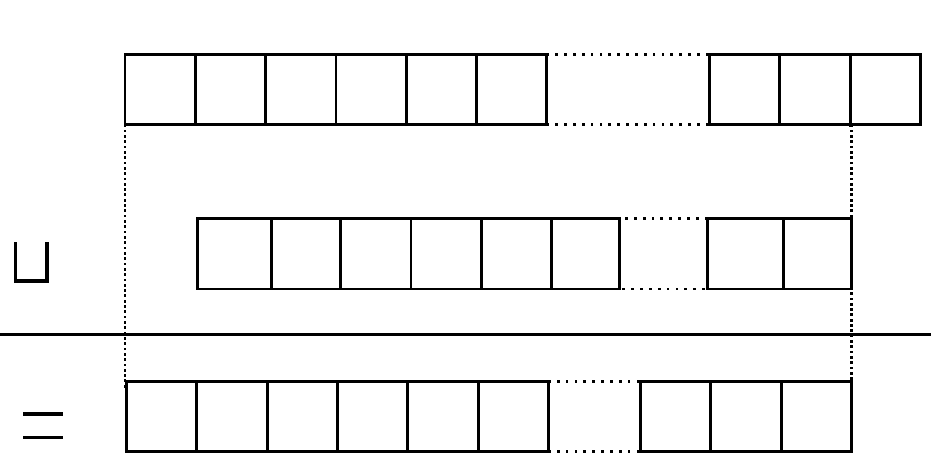
\includegraphics[width=7cm]{cuptype.pdf}
\vspace{0.2cm}
\hrule
    \caption{    \label{figsuptype}The supremum operator $\sqcup$ of  Equation (\ref{eqsuptype}).}
  \end{center}
\end{figure}


The function \texttt{unifyReal} calls in  a mutually recursive way the function \texttt{unify}
on terms. It also refers to type variables correspndig the constructor \texttt{TypeVar}.
The fields of \texttt{TypeVar} are the value itself and a string corrsponding to
the name of the variable. The value may be either \texttt{None} when the type
variable is not constrained or some reference to an expression when a type has been given to the variable
by unification. The function \texttt{solve} performs a partial evaluation of the expressions
occurring in the equations, in order to simplify them, translates them for \texttt{Z3},
calls the SMT solver and then assign the values of the solution to the relevant type
variables. The function \texttt{solveLT} acts just like the function \texttt{solve} but
requires that the precision of the second expression is greater than or equal to the precision of the first
expression instead of a strict equality.
Several cases are distinguished in the function \texttt{unifyReal} of Figure \ref{unireal}:
\begin{itemize}
\item If $\phi_1$ and $\phi_2$ are fully instantiated, i.e.  $s_i,u_i$ and $p_i$, $1\le i\le 2$
are integers then we assign $\phi=\phi_1 \sqcup\phi_2$ to $\phi_1$ and $\phi_2$.
The supremum $\sqcup$ refers to the order $\sqsubseteq$ introduced in  Equation (\ref{eqlttype}).
Formally, we have:
\begin{equation}\label{eqsuptype}
\phi_1\sqcup\phi_2=\big\{ s_1 \uplus s_2,\max(u_1,u_2),p\big\}\ \text{with}\ p=\left\{
\begin{array}{l}
\min(p_1,u_1-u_2+p_2)\ \text{if}\ u_1\ge u_2\enspace ,\\
\min(p_2,u_2-u_1+p_1)\ \text{otherwise}\enspace .
\end{array}\right.
\end{equation}
In Equation (\ref{eqsuptype}), $\uplus$ computes the supremum of to values of \textsf{Sign}.
Figure \ref{figsuptype} illustrates the effect of the operator $\sqcup$.
\item If $\phi_1$ is fully instantiated and $\phi_2$ is made of three type variables then $\phi_1$
is assigned to $\phi_2$.
\item If $\phi_1$ is fully instantiated and $\phi_2$ is neither fully instantiated or a triple
of type variables then $\phi-2$ is made of three integer expressions containing type variables,
$\phi_2=\{e_0,e_1,e_2\}$. We have to solve the system 
\begin{equation}
(S)\ : \ \left\{
\begin{array}{l}
s_1 = e_0\\
u_1 = e_1\\
p_1 = e_2
\end{array}\right.\enspace .
\end{equation}
We call the SMT solver \texttt{Z3} to solve this system of equation. Recall that $e_0$, $e_1$ and
$e_2$ come from the types of primitives introduced in Figure \ref{figtypprim}. These expressions
are linear and are easy to solve for an SMT solver.
\item If both $\phi_1$ and $\phi_2$ are made of type variables then we identify them in a pairwise
manner.
\item If both $\phi_1$ and $\phi_2$ are integer expressions then 
$\phi_1=\{e_0,e_1,e_2\}$ and $\phi_2=\{e'_0,e'_1,e'_2\}$. We have to solve the system 
\begin{equation}
(S)\ : \ \left\{
\begin{array}{l}
e_0 = e'_0\\
e_1 = e'_1\\
e_2 = e'_2
\end{array}\right.\enspace .
\end{equation}
Again, we call \texttt{Z3} to solve this system of linear equations.
\item The other cases are symmetric to the ones detailled formerly, they are treated similarly.
\end{itemize}


\begin{figure}[t]
\begin{center}\tt\scriptsize
\hrule
\vspace{0.2cm}
\begin{tabular}{lll}
\begin{lstlisting}[mathescape]
($\mathbf{assert}$ (= 2 
  ($\mathbf{ite}$ ($\mathbf{and}$ (= a 0) (= 1 0)) 0 
   ($\mathbf{ite}$ ($\mathbf{and}$ (= a 1) (= 1 1)) 1 
    ($\mathbf{ite}$ ($\mathbf{and}$ (= a -1) (= 1 -1)) -1 
     ($\mathbf{ite}$ ($\mathbf{and}$ (= a 1) (= 1 0)) 1 
      ($\mathbf{ite}$ ($\mathbf{and}$ (= a 0) (= 1 1)) 1
       ($\mathbf{ite}$ ($\mathbf{and}$ (= a -1) (= 1 0)) -1 
        ($\mathbf{ite}$ ($\mathbf{and}$ (= a 0) (= 1 -1)) -1 
         ($\mathbf{ite}$ ($\mathbf{and}$ (= a 1) (= 1 -1))
  ($\mathbf{ite}$ (> (+ ($\mathbf{ite}$ (>= b -7) b -7) 
   ($\mathbf{ite}$ ($\mathbf{and}$ (= a 0) (= 1 0)) 0 
    ($\mathbf{ite}$ ($\mathbf{and}$ (= a 1) (= 1 -1)) -1 
     ($\mathbf{ite}$ ($\mathbf{and}$ (= a -1) (= 1 1)) -1 
      ($\mathbf{ite}$ ($\mathbf{and}$ (= a -1) (= 1 -1)) 1 
       ($\mathbf{ite}$ ($\mathbf{and}$ (= a 1) (= 1 1)) 1 
        ($\mathbf{ite}$ ($\mathbf{and}$ (= a 1) (= 1 0)) 0 
         ($\mathbf{ite}$ ($\mathbf{and}$ (= a 0) (= 1 1)) 0
          ($\mathbf{ite}$ ($\mathbf{and}$ (= a -1) (= 1 0)) 0 
  ($\mathbf{ite}$ ($\mathbf{and}$ (= a 0) (= 1 -1)) 0
       2)))))))))) -7) 1 
   ($\mathbf{ite}$ (< (+ ($\mathbf{ite}$ (>= b -7) b -7) 
    ($\mathbf{ite}$ ($\mathbf{and}$ (= a 0) (= 1 0)) 0 
     ($\mathbf{ite}$ ($\mathbf{and}$ (= a 1) (= 1 -1)) -1 
      ($\mathbf{ite}$ ($\mathbf{and}$ (= a -1) (= 1 1)) -1 
       ($\mathbf{ite}$ ($\mathbf{and}$ (= a -1) (= 1 -1)) 1 
        ($\mathbf{ite}$ ($\mathbf{and}$ (= a 1) (= 1 1)) 1 
         ($\mathbf{ite}$ ($\mathbf{and}$ (= a 1) (= 1 0)) 0 
          ($\mathbf{ite}$ ($\mathbf{and}$ (= a 0) (= 1 1)) 0
  ($\mathbf{ite}$ ($\mathbf{and}$ (= a -1) (= 1 0)) 0 
    ($\mathbf{ite}$ ($\mathbf{and}$ (= a 0) (= 1 -1)) 0
         2)))))))))) -7) -1 2)) 
\end{lstlisting}
& &
\begin{lstlisting}[mathescape]
($\mathbf{ite}$ ($\mathbf{and}$ (= a -1) (= 1 1)) 
 ($\mathbf{ite}$ (< (+ ($\mathbf{ite}$ (>= b -7) b -7) 
  ($\mathbf{ite}$ ($\mathbf{and}$ (= a 0) (= 1 0)) 0 
   ($\mathbf{ite}$ ($\mathbf{and}$ (= a 1) (= 1 -1)) -1 
    ($\mathbf{ite}$ ($\mathbf{and}$ (= a -1) (= 1 1)) -1 
     ($\mathbf{ite}$ ($\mathbf{and}$ (= a -1) (= 1 -1)) 1 
      ($\mathbf{ite}$ ($\mathbf{and}$ (= a 1) (= 1 1)) 1 
       ($\mathbf{ite}$ ($\mathbf{and}$ (= a 1) (= 1 0)) 0 
        ($\mathbf{ite}$ ($\mathbf{and}$ (= a 0) (= 1 1)) 0
         ($\mathbf{ite}$ ($\mathbf{and}$ (= a -1) (= 1 0)) 0 
          ($\mathbf{ite}$ ($\mathbf{and}$ (= a 0) (= 1 -1)) 0
            2)))))))))) -7) 1 
 ($\mathbf{ite}$ (> (+ ($\mathbf{ite}$ (>= b -7) b -7) 
  ($\mathbf{ite}$ ($\mathbf{and}$ (= a 0) (= 1 0)) 0 
   ($\mathbf{ite}$ ($\mathbf{and}$ (= a 1) (= 1 -1)) -1 
    ($\mathbf{ite}$ ($\mathbf{and}$ (= a -1) (= 1 1)) -1 
     ($\mathbf{ite}$ ($\mathbf{and}$ (= a -1) (= 1 -1)) 1 
      ($\mathbf{ite}$ ($\mathbf{and}$ (= a 1) (= 1 1)) 1 
       ($\mathbf{ite}$ ($\mathbf{and}$ (= a 1) (= 1 0)) 0 
        ($\mathbf{ite}$ ($\mathbf{and}$ (= a 0) (= 1 1)) 0
         ($\mathbf{ite}$ ($\mathbf{and}$ (= a -1) (= 1 0)) 0 
          ($\mathbf{ite}$ ($\mathbf{and}$ (= a 0) (= 1 -1)) 0
            2)))))))))) -7) -1 2))
     2)))))))))))
\end{lstlisting}
\end{tabular}
\vspace{0.2cm}
\hrule
\end{center}
\caption{\label{figz3}\texttt{Z3} encoding of the first equality of Equation (\ref{exsmteq}).}
\end{figure}

For example, the equations sent to the SMT solver for 
the call \texttt{newton 9.0 0.0 g gprime ;;} to 
the  \texttt{newton} function
of Section \ref{over} are given in Equation (\ref{exsmteq}).

\begin{equation}\label{exsmteq}
(S)\ :\ \left\{
\begin{array}{l}

\mathcal{S}_+( \mathtt{'a}, \max( \mathtt{'b}, -7) + \mathcal{S}_\times( \mathtt{'a}, 1), 1, -7)=2\\
\ \\
(\max (\mathtt{'b}, -7) + \mathcal{S}_\times (\mathcal{S}_+ (\mathtt{'a}, \mathtt{'b}, 1, -7), 1)=10\\
\ \\
\max (\max( \mathtt{'b}, -7) + \mathcal{S}_\times (\mathcal{S}_+ (\mathtt{'a}, \mathtt{'b}, 1, -7), 1), -7) \\
+ 
\mathcal{S}_\times (\mathcal{S}_+ (\mathtt{'a}, \max (\mathtt{'b}, -7) + \mathcal{S}_\times( \mathtt{'a}, 1), 1, -7), 1)\\ 
- \max (\max( \mathtt{'b}, -7) + \mathcal{S}_\times (\mathcal{S}_+(\mathtt{'a}, \mathtt{'b}, 1, -7), 1) - \mathtt{'c}, -60)\\ 
- \iota (\max (\mathtt{'b}, -7) + \mathcal{S}_\times (\mathcal{S}_+( \mathtt{'a}, \mathtt{'b}, 1, -7) ,1) - \mathtt{'c} ,-60)
\le 21
\end{array}\right.
\end{equation}
These equations are encoded in \texttt{Z3} by expanding the operators $\max$, $\mathcal{S}_+$,
$\mathcal{S}_\times$, and $\iota$ following the definitions of Figure \ref{figtypprim}.
For example, the \texttt{Z3} encoding of the first equality of
Equation (\ref{exsmteq}) is displayed in Figure \ref{figz3}. Globally, the encoding of the three
equations of Equation (\ref{exsmteq}) is a $1007$ lines long \texttt{Z3} file.
\texttt{Z3} solves these equations in $0.215$ seconds (average measured time on $5$ executions).



\subsection{Experiments}
\label{morex}



\section{Case of the IEEE754 Floating-Point Arithmetic}
\label{ieee}

In this section, we introduce modified versions of the types of primitives introduced in Section
\ref{secdefprim}. These modified versions are specific to the IEEE754 floating-point arithmetic \cite{IEEE754}.
The types introduced in Figure \ref{figtypprim} for the primitives corresponding to the elementary operations
$+$, $-$, $\times$ and $\div$ are not tailored for a specific arithmetic. They only assume
that the system has enough bits to perform the operations in the format given by
the types so that the results of the operations are not rounded. \texttt{Numl} interpreter 
fulfills this requirement by performing all the numerical computations in multiple precision,
using the GNU Multiple Precision Arithmetic library \texttt{GMP}.
Indeed, the type inference enables to determine \textit{a priori} the precision needed by \texttt{GMP} for the
values and arithmetic operations. An optimization would consists of also detecting when the
computations fit into hardware formats (generally the formats of the IEEE754 arithmetic introduced in Figure
\ref{formats}) in order to avoid the calls to \texttt{GMP} when possible. The type information
also permits to generate code for the fixed-point arithmetic \cite{MENTOR}. In this case,
if the precision of the formats corresponds to the types, no additional roundoff errors have to be added
and the general equations of Figure \ref{figtypprim} hold again.
In future work, we plan to develop a compiler for our language (in addition to the current interpreter)
which, based on the formats given by the types,  generates code using either the IEEE754 or the multiple precision arithmetic (only when necessary).
This compiler would also generate code for the fixed-point arithmetic. 


\begin{figure}[tb]
\hrule			
$$
\begin{array}{c}
\varrho\in\{11,24,53,113\}\\
\\
\mathcal{P}_+^\varrho(\mathtt{s_1},\mathtt{u_1},\mathtt{p_1},\mathtt{s_2},\mathtt{u_2},\mathtt{p_2}) =\\
\\
(\mathtt{u_1},\mathtt{u_2})+\sigma_+(\mathtt{s_1},\mathtt{s_2})-
\max\left(\begin{array}{c}
\mathtt{u_1}-\mathtt{p_1},\\
\mathtt{u_2}-\mathtt{p_2},\\
\mathcal{U}_{+}(\mathtt{s_1},\mathtt{u_1},\mathtt{s_2},\mathtt{u_2})-\varrho
\end{array}\right)
-\iota_3
\left(\begin{array}{c}
\mathtt{u_1}-\mathtt{p_1},\\
\mathtt{u_2}-\mathtt{p_2},\\
\mathcal{U}_{+}(\mathtt{s_1},\mathtt{u_1},\mathtt{s_2},\mathtt{u_2})-\varrho
\end{array}\right)
\\
\\
\\
\begin{array}{c}
\mathcal{P}_-^\varrho(\mathtt{s_1},\mathtt{u_1},\mathtt{p_1},\mathtt{s_2},\mathtt{u_2},\mathtt{p_2}) =\\
\\
(\mathtt{u_1},\mathtt{u_2})+\sigma_-(\mathtt{s_1},\mathtt{s_2})- 
\max\left(\begin{array}{c}
\mathtt{u_1}-\mathtt{p_1},\\
\mathtt{u_2}-\mathtt{p_2},\\
\mathcal{U}_{-}(\mathtt{s_1},\mathtt{u_1},\mathtt{s_2},\mathtt{u_2})-\varrho
\end{array}\right)
-\iota_3
\left(\begin{array}{c}
\mathtt{u_1}-\mathtt{p_1},\\
\mathtt{u_2}-\mathtt{p_2},\\
\mathcal{U}_{-}(\mathtt{s_1},\mathtt{u_1},\mathtt{s_2},\mathtt{u_2})-\varrho
\end{array}\right)
\end{array}
\\
\\
\\
\mathcal{P}_\times^\varrho(\mathtt{s_1},\mathtt{u_1},\mathtt{p_1},\mathtt{s_2},\mathtt{u_2},\mathtt{p_2}) = \\
\\
\mathtt{u_1}+\mathtt{u_2}+1-
\max\left(\begin{array}{c}
\mathtt{u_1}+\mathtt{u_2}+1-\mathtt{p_1},\\
\mathtt{u_1}-\mathtt{u_2}+1-\mathtt{p_2},\\
\mathtt{u_1}-\mathtt{u_2}+1-\varrho
\end{array}\right)
-\iota_3
\left(\begin{array}{c}
\mathtt{u_1}+\mathtt{u_2}+1-\mathtt{p_1},\\
\mathtt{u_1}-\mathtt{u_2}+1-\mathtt{p_2},\\
\mathtt{u_1}-\mathtt{u_2}+1-\varrho
\end{array}\right)
\\
\\
\\
\mathcal{P}_\div^\varrho(\mathtt{s_1},\mathtt{u_1},\mathtt{p_1},\mathtt{s_2},\mathtt{u_2},\mathtt{p_2})=
\mathcal{P}_\times^\varrho(\mathtt{u_1},\mathtt{p_1},\mathtt{u_2},\mathtt{p_2})\\
\\
\\
\iota_3(x,y,z)=\left\{\begin{array}{l}
1 \ \text{if}\ x=y\ \vee\ x=z\ \vee\ y=z,\\
0\ \text{otherwise}.
\end{array}\right.
\end{array}
$$
\hrule
\caption{\label{prim754}Types of the IEEE754 floating-point arithmetic operators in precision $\varrho$.} 
\end{figure}




In practice, in many cases, one wants to use the IEEE754 floating-point arithmetic and not
multiple precision libraries, for efficiency reasons or because these library are not available in
certain contexts. In this case, the values and the results of the operations do not
necessarily  fit inside the IEEE754 formats of Figure \ref{formats}, they must be rounded. 
The IEEE754 Standard defines five rounding modes for elementary operations over
floating-point numbers. These modes are towards $-\infty$, towards $+\infty$, towards zero,
 to the nearest ties to even and to the nearest ties to away and we write them $\circ_{-\infty}$, $\circ_{+\infty}$, $\circ_0$, 
$\circ_{\sim_e}$ and $\circ_{\sim_a}$, respectively.
The semantics of the elementary operations $\ast\in\{+,\ -,\ \times,\ \div\}$  is then defined by
\begin{equation}
\label{roundoff}\small
f_1\ \ast_{\circ}\ f_2\ =\ \circ\ (f_1\ \ast\ f_2) 
\end{equation}
%
where $\circ\in\{\circ_{-\infty},\circ_{+\infty},\circ_{0},\circ_{\sim_e},\circ_{\sim_a}\}$ denotes the rounding mode.
Equation (\ref{roundoff}) states that the result of a floating-point operation $\ast_\circ$ done
with the rounding mode $\circ$ returns what we would obtain by performing the exact operation $\ast$
and next rounding the result using $\circ$.
The IEEE754 Standard also specifies how the square root function must be rounded in a similar way
to Equation (\ref{roundoff}) but does not specify
the roundoff of other functions like sin, log, etc.


In the IEEE754 arithmetic, additional errors arise compared to the general context of Section \ref{secdefprim} and 
the types of the primitives of Figure \ref{figtypprim}
must be modified to correctly model the errors of this specific arithmetic.
The types of the IEEE754 primitives in precision $\varrho\in \{11,24,53,113\}$, i.e. in half, single,
double or quadruple precision, is given in Figure \ref{prim754}. We assume that the
rounding mode is  $\sim\in\{\sim_a,\sim_e\}$ (to the nearest.)
These equations model the fact that the accuracy of the result is dominated by either the error on
first operand or on the second operand or on the rounding of the result in precision $\varrho$.
For example, the error on $x+_\sim y$ is $e_+=\eps(x)+\eps(y)+\circ(x+y)$ with, by Equation (\ref{roundoff}),
\begin{equation}
\circ(x+y)< \frac{1}{2}\mathsf{ulp}(x+y)=\frac{1}{2}\mathsf{ufp}(x+y)-\varrho\enspace .
\end{equation}
The types of the other operators are obtained in a similar way to the addition.
Let us also note that in the IEEE754 floating-point arithmetic the constants may no longer
be in any precision. They must fit one of the formats given the standard.






\section{Related Work}
\label{relate}

Several approaches have been proposed to determine the best floating-point formats  as a function of the
expected accuracy on the results. Darulova and Kuncak use a forward static analysis to compute the propagation of errors
\cite{DK14}. If the computed bound on the accuracy satisfies the post-conditions then the analysis is
run again with a smaller format until the best format is found. Note that in this approach, all the values have
the same format (contrarily to our framework where each control-point has its own format).
While Darulova and Kuncak develop their own static analysis, other static techniques \cite{Gou13,Sal15} could be used to
infer from the forward error propagation the suitable formats. 
Chiang \textit{et al.} \cite{Call17} have proposed a method to allocate a precision to the terms of an arithmetic expression (only).
They use a formal analysis via Symbolic Taylor Expansions and
error analysis based on interval functions. 
In spite of our linear constraints, they solve a quadratically constrained quadratic program to obtain
 annotations.

Other approaches rely on dynamic analysis. For instance, the Precimonious tool tries to decrease the precision
of variables and checks whether the accuracy requirements are still fulfilled \cite{Nal16,Ral13}.
Lam \textit{et al} instrument binary codes in order to modify their precision without modifying the
source codes \cite{Lal13}. They also propose a dynamic search method to identify the pieces of code where the precision
should be modified.

Finally other work focus on formal methods and numerical analysis.
A first related research direction concerns formal proofs and the use of proof assistants to guaranty
the accuracy of finite-precision computations \cite{Bol15,Har07,Lee18}.
Another related research direction concerns the  compile-time optimization of programs in order to improve
the accuracy of the floating-point computation in function of given ranges for the inputs, without
modifying the formats of the numbers \cite{DMC15,Pal15}.

\section{Conclusion}
\label{conc}

In this article, we have introduced a dependent type system able to infer the accuracy of numerical computations.
This type system uses a modified Hindley-Milner algorithm which calls a SMT solver to solve linear
equations among integers to compute the accuracy information. Our type system allows one to type non-trivial 
programs corresponding to implementations of classical numerical analysis methods. Unstable computations
are rejected by the type system. The consistency of typed programs is ensured by a subject reduction theorem.

To our knowledge, this is the first type system dedicated to numerical accuracy. 
We believe that this approach has many advantages going from early debugging to
compiler optimizations. Indeed, we believe that the usual type \texttt{float} proposed by usual
\texttt{ML} implementations, and which is a simple clone of the type \texttt{int}, is too poor for numerical computations.
We also believe that this approach is a credible alternative to static analysis techniques for
numerical precision \cite{DK14,Gou13,Sal15}.
From the developper point of view, our type system
introduces few changes in the programming style, limited to giving the
accuracy of the inputs of the accuracy of comparisons to allow the typing of certain recursive functions.

A first perspective is to improve our type system in order to accept even more programs.
We would like to extend our language to mathematic elementary functions such as
$\log$, $\sin$, etc. But we would also like to explore more fundamental directions.
In some cases, there exists many solutions to the equations sent to \texttt{Z3}
and the solution given by the solver is not always the most appropriate one. Even if the
typing of a first expression $e$ is correct, other types were acceptable and the choice operated by the SMT solver
may be incompatible with the typing of other expressions who will call $e$ in the future.
To overcome this limitation, we plan to modify  our type inference algorithm to postpone as much as
possible the call to \texttt{Z3}.

A second perspective to the present work is the implementation of a compiler for \texttt{Numl}.
We aim at using the type information to select the most appropriate formats (the IEEE754 formats
of Figure \ref{formats}, multiple precisions numbers of the GMP library when needed or requested
by the user or fixed-point numbers.) At longer term, we also aim at introducing 
safe compile-time optimizations based on type preservation: an expression may be safely (from the
accuracy point of view) substituted to
another expression as long as both expressions are mathematically equivalent and that the
new expression has a greater type than the older one in the sense of Equation (\ref{eqlttype}).

Finally, a third perspective is to integrate our type system into other applicative
languages. In particular, it would be of great interest to have such a type system inside
a language used to build critical embedded systems such as the synchronous language \texttt{Lustre} \cite{Cal87}. 
In this context
numerical accuracy requirements are strong and difficult to obtain.
Our type system could be integrated naturally inside \texttt{Lustre} or similar languages.








%\begin{acks}
%This work is
%supported by the \grantsponsor{GS501100001809}{Office for Naval Research Global}
%{https://www.onr.navy.mil/Science-Technology/ONR-Global.aspx} under Grant
%No.: ̃\grantnum[http://www.nnsf.cn/youngscientists]{GS501100001809}{Tycoon}.
%\end{acks}

\bibliographystyle{ACM-Reference-Format}
\bibliography{main}

\end{document}

